\documentclass[AMA,STIX1COL]{WileyNJD-v2}\usepackage[]{graphicx}\usepackage[]{xcolor}
% maxwidth is the original width if it is less than linewidth
% otherwise use linewidth (to make sure the graphics do not exceed the margin)
\makeatletter
\def\maxwidth{ %
  \ifdim\Gin@nat@width>\linewidth
    \linewidth
  \else
    \Gin@nat@width
  \fi
}
\makeatother

\definecolor{fgcolor}{rgb}{0.345, 0.345, 0.345}
\newcommand{\hlnum}[1]{\textcolor[rgb]{0.686,0.059,0.569}{#1}}%
\newcommand{\hlstr}[1]{\textcolor[rgb]{0.192,0.494,0.8}{#1}}%
\newcommand{\hlcom}[1]{\textcolor[rgb]{0.678,0.584,0.686}{\textit{#1}}}%
\newcommand{\hlopt}[1]{\textcolor[rgb]{0,0,0}{#1}}%
\newcommand{\hlstd}[1]{\textcolor[rgb]{0.345,0.345,0.345}{#1}}%
\newcommand{\hlkwa}[1]{\textcolor[rgb]{0.161,0.373,0.58}{\textbf{#1}}}%
\newcommand{\hlkwb}[1]{\textcolor[rgb]{0.69,0.353,0.396}{#1}}%
\newcommand{\hlkwc}[1]{\textcolor[rgb]{0.333,0.667,0.333}{#1}}%
\newcommand{\hlkwd}[1]{\textcolor[rgb]{0.737,0.353,0.396}{\textbf{#1}}}%
\let\hlipl\hlkwb

\usepackage{framed}
\makeatletter
\newenvironment{kframe}{%
 \def\at@end@of@kframe{}%
 \ifinner\ifhmode%
  \def\at@end@of@kframe{\end{minipage}}%
  \begin{minipage}{\columnwidth}%
 \fi\fi%
 \def\FrameCommand##1{\hskip\@totalleftmargin \hskip-\fboxsep
 \colorbox{shadecolor}{##1}\hskip-\fboxsep
     % There is no \\@totalrightmargin, so:
     \hskip-\linewidth \hskip-\@totalleftmargin \hskip\columnwidth}%
 \MakeFramed {\advance\hsize-\width
   \@totalleftmargin\z@ \linewidth\hsize
   \@setminipage}}%
 {\par\unskip\endMakeFramed%
 \at@end@of@kframe}
\makeatother

\definecolor{shadecolor}{rgb}{.97, .97, .97}
\definecolor{messagecolor}{rgb}{0, 0, 0}
\definecolor{warningcolor}{rgb}{1, 0, 1}
\definecolor{errorcolor}{rgb}{1, 0, 0}
\newenvironment{knitrout}{}{} % an empty environment to be redefined in TeX

\usepackage{alltt}
\articletype{Research Article}%

\received{}
\revised{}
\accepted{}

\usepackage{graphicx}
\usepackage{booktabs}
\usepackage{alltt}
\usepackage{amsmath}
\usepackage{longtable}
\usepackage{algorithm}
\usepackage{algpseudocode}
\usepackage{threeparttable}
\usepackage{verbatim}
\usepackage{bm}
\usepackage{enumerate}
\usepackage{multirow}


\usepackage{hyperref}
\hypersetup{
    colorlinks=true,
    linkcolor=blue,
    filecolor=blue,
    urlcolor=blue,
    citecolor=blue,
    }

% My definitions

\newcommand{\R}{R}
\newcommand{\gbsg}{gbsg}
\def\FsNg{\hbox{FS-M}}

\def\hhat{\hat\theta(\widehat{H})}
\def\hchat{\hat\theta(\widehat{H}^{c})}

\def\hhatB{\hat\theta^{*}(\widehat{H})}
\def\hchatB{\hat\theta^{*}(\widehat{H}^{c})}


\def\hknow{\hat\theta(H)}
\def\hcknow{\hat\theta(H^{c})}

\def\hplim{\theta^{\dagger}(H)}
\def\hcplim{\theta^{\dagger}(H^{c})}
\def\hplimitt{\theta^{\dagger}(\hbox{ITT})}

\def\fsl{FS_{l}}
\def\fslg{FS_{lg}}
\def\grfa{GRF}
\def\grfb{GRF_{60}}


\def\hhplim{\theta^{\ddagger}(H)}
\def\hhcplim{\theta^{\ddagger}(H^{c})}

\def\Hhplim{\theta^{\ddagger}(\widehat{H})}
\def\Hhcplim{\theta^{\ddagger}(\widehat{H}^{c})}

\def\hath{\widehat{H}}
\def\hathc{{\widehat{H}}^{c}}

\startpage{1}
\raggedbottom
\IfFileExists{upquote.sty}{\usepackage{upquote}}{}
\begin{document}

\title{Exploratory subgroup identification in the heterogeneous Cox model: A relatively simple procedure}
\author[1]{Larry F. Le\'on}
\author[1]{Thomas Jemielita}
\author[2]{Zifang Guo}
\author[1]{Rachel Marceau West}
\author[1]{Keaven M. Anderson}

\authormark{Larry F. Le\'on \textsc{et al}}
\titlemark{Exploratory subgroup identification in the heterogeneous Cox model: A relatively simple procedure}

\address[1]{\orgdiv{Biostatistics and Research Decision Sciences}, \orgname{Merck \& Co., Inc.}, \orgaddress{\state{New Jersey}, \country{USA}}}
\address[2]{\orgdiv{Biostatistics}, \orgname{BioNTech SE}, \orgaddress{\state{New York}, \country{USA}}}

\corres{*Larry F. Le\'on, Biostatistics and Research Decision Sciences, Merck \& Co., Inc., Rahway, New Jersey, USA \email{larry.leon2@Merck.com}}


\abstract[Abstract]{
For survival analysis applications we propose a novel procedure for identifying subgroups with large treatment effects, with focus on subgroups where treatment is potentially detrimental.  The approach, termed forest search, is relatively simple and flexible.  All-possible subgroups are screened and selected based on hazard ratio thresholds indicative of harm with assessment according to the standard Cox model. By reversing the role of treatment one can seek to identify substantial benefit. We apply a splitting consistency criteria to identify a subgroup considered “maximally consistent with harm”.  
The type-1 error and power for subgroup identification can be quickly approximated by numerical integration. To aid inference we describe a bootstrap bias-corrected Cox model estimator with variance estimated by a jacknife approximation.  We provide a detailed evaluation of operating characteristics in simulations and compare to virtual twins and generalized random forests where we find the proposal to have favorable performance.  In particular, in our simulation setting, we find the proposed approach favorably controls the type-1 error for falsely identifying heterogeneity with higher power and classification accuracy for substantial heterogeneous effects. Two real data applications are provided for publicly available datasets from a clinical trial in oncology, and HIV.
}

\keywords{Censored data; generalized random forests; virtual twins; bootstrap bias-correction, cross-validation}

\maketitle

\section{Introduction}\label{sec:intro}

In oncology trials subgroup analyses via forest plots are standard presentations in regulatory reviews and clinical publications with the goal of evaluating the consistency of treatment effects across the pre-specified subgroups relative to the intention-to-treat (ITT) population.   The European Medicines Agency guideline on subgroups \cite{EMA_2019} further describes scenarios where there is interest ``to identify post-hoc a subgroup where efficacy and risk-benefit is convincing'' or ``in identifying a subgroup, where a relevant treatment effect and compelling evidence of a favorable risk-benefit profile can be assessed''.   In a recent review of regulatory considerations for case examples in oncology Amatya et al \cite{AT_2021} discuss approvals in the ``ITT population despite decreased treatment effect in an important subgroup'' as well as approvals in subgroups.  The underlying theme in these regulatory reviews was the assessment of an apparent detrimental effect, the evidence for potential harm and biological plausibility.    

While pre-specified subgroups provide a higher level of evidence than post-hoc analyses there could be important subgroups based on patient characteristics that are not anticipated or well understood.  We investigate approaches for exploratory subgroup identification in survival analysis applications with the goal of identifying an underlying subgroup, $H$ say, consisting of subjects who derive the least benefit from treatment.  Ideally subgroup identification would be attempted in Phase 2 in order to inform Phase 3 study design and analysis considerations.  In this work we focus on large effects (negative or positive) as “lack of benefit or mild benefit” may not be sufficient reason to recommend against treatment or to exclude from inclusion in future program development.  In the case of an existing detrimental $H$, the complementary population $H^{c}$ may potentially be considered to derive benefit with a “higher degree of confidence” relative to the overall ITT population.  

The novel methodology in this research, termed forest search (FS), is based on extending the idea of all-possible subsets of covariate regression models from the area of model selection to evaluating all-possible subgroups formed by combinations of baseline candidate factors.  For the selection of candidate factors any well-defined algorithm can be applied.  As a ``base-case'' algorithm we consider generalized random forests,\cite{ATW_2019,AW_2021,CZ_2023} henceforth GRF, as a core component which we use with or without lasso.\cite{SFHT_2011}  GRF is a subgroup identification approach itself based on restricted mean survival time summaries via causal survival forests, whereas lasso estimates the Cox model via regularization.  In our applications we illustrate various combinations of GRF and lasso, including evaluating all baseline factors with continuous covariates cut at the quartiles.  For identified subgroups, $\hath$ and $\hathc$ say, inference based on bootstrap bias-corrected estimators is described which accounts for the overall FS algorithm including the manner in which candidate factors are selected.  While we are directly targeting identification of $H$, the primary goal of inference can be with regard to $H^{c}$.  In addition, by reversing the roles of treatment (switching the treatment indicator) the identification of ``harm'' can be formulated to identify substantial benefit which will be illustrated in our second real data application.  To evaluate the quality and stability of the FS algorithm(s) we propose two forms of cross-validation.

For identifying $H$ we define initial candidates as subgroups with Cox hazard ratio estimates $\geq 1.25$ (experimental-vs-control) and employ the following splitting consistency criteria.  Here Cox hazard ratio estimates correspond to the standard model (adjusted for treatment only) applied within the subgroup which is common in standard forest plot summaries in oncology trials. Suppose there are subgroups with estimates $\geq 1.25$ and for each subgroup we randomly split the subgroup (in half) many times and consider each split consistent with harm if the estimated hazard ratio is $\geq 1.0$ for each of the two subgroup splits.  We define $H$-candidates as those with consistency rates at least $90\%$ and define the estimated subgroup, $\hath$ say, as the subgroup with the highest consistency rate; $\hath$ is considered “maximally consistent with harm” and $\hathc$ is the complement.  If no subgroup achieves a consistency rate of at least $90\%$ then define $\hath$ as null with $\hathc$ the ITT population. The consistency criteria heuristically represents --“no matter how you split the subgroup $\hath$, those splits are both generally consistent with harm”.  The choice of the screening and consistency thresholds ($1.25$ and $1.0$, respectively) is based on power approximations and confirmed in simulations to control the false-discovery of $H$-subgroups and have reasonable ability to detect existing subgroups with large (detrimental) effects.   The splitting consistency criteria is similar in spirit to cross-validation, however our goal is not prediction evaluation, but rather to have independent assessments for evidence of harm which is provided by both (independent) random splits having hazard ratio estimates $\geq 1.0$ across repeated sample splitting.  

Our work is closely related to Guo et al\cite{GH2021} who consider inference for the largest treatment effect across pre-specified subgroups.  However, the FS algorithm for maximizing the consistency rate does not necessarily correspond to the largest observed treatment effect estimate.  Moreover, crucially, we are not pre-specifying a limited set of subgroups but searching for subgroups across a large collection of combinations, conceptually a large forest plot.  We refer to Dandl et al\cite{Dandl_2024} for a recent review of forest-based approaches (see also Knaus\cite{Knaus_2022}), as well as Ballarini et al\cite{Ballarini_2021} for a summary of additional approaches and statistical software.  

As a practical illustration we consider a simulated dataset generated as described in Section \ref{sec:sims} which included 7 baseline factors of which 5 were 
prognostic ($Z_1-Z_5$, say) and the other 2 non-prognostic ($Z_6$, $Z_7$) but correlated with the prognostic factors.  In addition, 3 independent $N(0,1)$ random noise variables ($Z_8$, $Z_9$, $Z_{10}$) were included for a total of 10 baseline factors; 
consisting of 6 binary (first 6) and 4 continuous factors.  We define random noise variables as baseline factors which are completely unrelated to the outcome data-generating process.  The underlying subgroup $H$ was an interaction between $Z_1$ and $Z_3$ (subjects with $Z_1=1$ and $Z_3=1$).  In this simulated example there were $N=1000$ subjects, randomized 1:1, with an observed censoring of approximately $45\%$.  The underlying marginal hazard ratio for the harm population $H$ was $\hplim =2$ (say), and for the complement $\hcplim =0.65$; the number of subjects in the $H$ and $H^{c}$ subgroups was $116$ and $884$, respectively.  The ITT Kaplan-Meier curves displayed in Figure {\ref{fig1}}exhibit a delayed treatment effect pattern with lack of separation roughly in the first 12 months; the Cox model estimates ($95\%$ CI) were $0.73$ ($0.62$, $0.87$).


\begin{figure*}[h]
\begin{center}
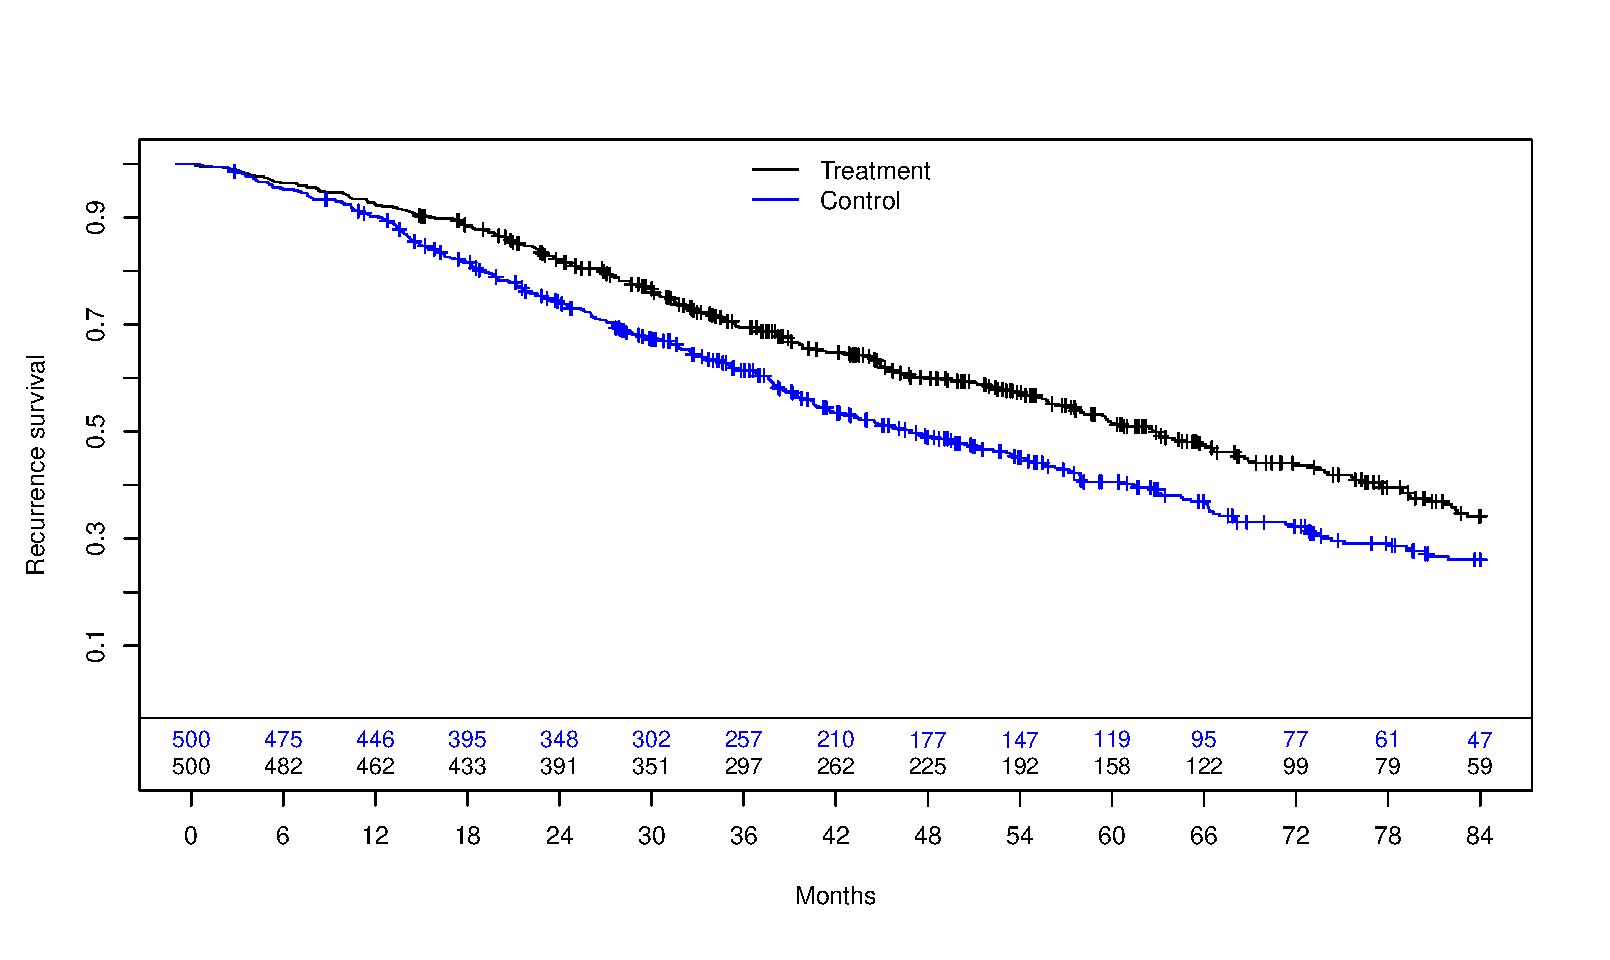
\includegraphics[width=5.5in, height=3.25in]{Figure 1.eps}
\end{center}
\caption{Kaplan-Meier curves for simulated dataset (intention-to-treat population).}
\label{fig1}
\end{figure*}


To explore subgroups we proceed as follows. Suppose we cut the continuous variables at the medians so that there are 10 binary factors and $L=20$ subgroup indicators (further described in section \ref{sec:SIA}).  There would then be over 1 million all-possible subgroup combinations ($2^{L} -1$).  However for practical considerations we restrict to subgroups formed by a maximum of two factors which is analogous to ``tree depths'' in random forests (In practice, it may be difficult to clinically interpret subgroups based on 3 or more factors.).  Among two-factor combinations there are $L(L-1)/2+L = 400$ possible subgroup combinations.  We also restrict to subgroups with at least 60 subjects (approximately $30$ subjects per arm under 1:1 randomization) and 10 events in each arm which we consider minimal sample size requirements for Cox model applications. In addition, we apply lasso and GRF for selection of continuous variables and splits thereof.  The application of lasso selected $Z_1$, $Z_4$, $Z_5$, $Z_6$, and $Z_8$, which captured only 3 ($Z_1, Z_4,$ and $Z_5$ which are binary) of the truly prognostic factors and crucially excluded $Z_3$ which defined (along with $Z_1$) the true subgroup.  GRF selected $Z_1$, $Z_3$ and $Z_8$ (split at $\leq 0.89$) as candidates.   In this example lasso was somewhat aggressive in excluding factors but the incorporation of GRF re-introduced $Z_3$. For $Z_6$ (selected by lasso) this was cut at the median.  Both lasso and GRF selected the random noise (continuous) factor $Z_8$, for which the cut $Z_8 \leq 0.89$ was used per GRF, and neither selected the prognostic factor $Z_2$.  In total FS evaluated 6 binary factors ($X_1=Z_1$, $X_2=Z_3$, $X_3=Z_4$, $X_4=Z_5$, $X_5=(Z_6 \leq \hbox{med}(Z_6))$, and $X_6=(Z_8 \leq 0.89)$, say) where the number of all-possible combinations was $12(11/2)+12 = 78$, of which 70 subgroups satisfied the aforementioned sample size criteria.   

The estimated $H$ subgroup was the true subgroup and thus Cox model estimates correspond to the oracle estimator where the true subgroup was known a-priori.  The Cox estimates (FS and oracle) were $2.36$ ($1.53$, $3.66$) for $\hath$, and $0.63$ ($0.52$, $0.76$) for $\hathc$.  While these confidence intervals would be valid for the oracle estimator pretending the true subgroup is pre-specified, the FS estimator requires adjustment for the overall procedure.  Applying our bootstrap approach the bias-corrected estimates were $2.04$ ($1.19$, $3.47$) for $\hath$, and 
$0.63$ ($0.48$, $0.83$) for $\hathc$.

The manner of choosing candidate factors (binary splits) is not restricted to the above GRF and lasso algorithm.  In our applications we also consider GRF along with cutting all continuous factors at the mean, median, 
1st quartile ($q_1$), and 3rd quartile ($q_3$), where lasso is not included in the algorithm (i.e., four splits for each continuous factor).  For example, with 6 binary and 4 continuous factors there would be $L=44$ subgroup indicators ($22$ binary factors) and $990$ possible two-factor subgroup combinations.  In addition, one can first apply lasso and then cut all (lasso selected) continuous factors in the above manner.  Whichever candidate selection algorithm 
is employed the bootstrap process for bias-correction and variance estimation would incorporate the algorithm, mimicking the entire procedure.  To evaluate the quality and stability of the chosen algorithm, and to compare algorithms (e.g., with or without lasso),  we propose two forms of cross-validation. 

This paper is organized as follows.  In Section \ref{sec:SIA} we describe our proposal for subgroup identification along with an asymptotic approximation for the power to identify (any) $H$ which is the basis for the choice of the FS hazard ratio thresholds ($1.25$ for screening and $1.0$ for consistency).  In simulations, Section \ref{sec:sims}, we compare operating characteristics of the proposed FS approach to virtual twins \citep{FTR_2011} and generalized random forests \cite{ATW_2019,AW_2021,CZ_2023} in terms of identification (type-1 error and power) and classification accuracy for correctly identifying subjects in $H$ and $H^{c}$.  Performance of the bootstrap bias-corrected FS estimators are also evaluated.  In Section \ref{sec:applications} we introduce the cross-validation approach for evaluating the quality and stability of the FS algorithm with 
two real data applications, the German Breast Cancer Study Group trial data \cite{Schumacher_1994}, and the ACTG-175 HIV trial.\cite{ACTG175}  A summary discussion is provided in Section \ref{sec:discuss}.  Additional details are provided in the Supplementary materials.






\section{Subgroup Identification Approach} \label{sec:SIA}

We consider the two-sample random censorship model with $N$ observations from a randomized clinical trial.
Let $T$ denote the survival time, $C$ the censoring time, $V$ the treatment assignment, 
and $Z=(Z_{1},Z_{2},\ldots,Z_{p})$ a $p$-dimensional collection of baseline covariates.  It is of interest to evaluate subgroups 
formed by combinations of these baseline covariates. We observe the possibly
censored survival time $Y=\min(T,C)$ with $\Delta=I(T \leq C)$ the event indicator. 
The survival times $T$ and censoring times $C$ are assumed to be independent, conditional on $(V,Z)$, with continuous distributions. The observations $(V_{i},Z_{i},Y_{i},\Delta_{i})$ for $i=1,\ldots,N$ are assumed to be iid replicates.

In oncology trials the gold-standard primary ITT analysis is a Cox model with only the treatment arm as a covariate, usually stratified.\cite{ACR_2015,FK_2019}  Standard forest plots often proceed by fitting 

\begin{equation}
\lambda(t;V) = \lambda_{0}(t) \exp(\beta V),
\label{coxsg}
\end{equation}

\noindent within the subgroup levels of interest (e.g., by males and females separately).

In this work we assume heterogeneous treatment effects are induced by the existence of a detrimental subgroup $H$ with true marginal hazard ratio $\hplim > 1$ where the size of $H$ is at least $60$ subjects with an underlying expected event count $d$.  In our context there are two type-1 error scenarios for false subgroup identification: (i) If a subgroup $H$ is identified where in truth $\theta^{\dagger}(H) \leq 1$ (non-detrimental); and (ii) If the treatment effect is uniformly beneficial, $\hplimitt < 1$.   Under scenario (i) it is possible for 
heterogeneous treatment effects to exists (via mixture of true $H$ and $H^{c}$), but the composition of the identified subgroup $H$ is such that treatment is non-detrimental for the sub-population ($\hplim \leq 1$); in contrast under (ii) there does not exist such subgroup effects.
In the following section (\ref{sec:asymptotics}) we represent hazard ratio estimators based on a subgroup, and random splits thereof, via two normal random variables where the joint probability of meeting the screening and splitting consistency criterion thresholds is calculated by numerical integration.  Specifically, let $W_1$ and $W_2$ be two (independent) $N(\log(\hplim),8/d)$ random variables and define $p(c_1,c_2; d, \hplim) = \Pr(W_1+W_2 \geq 2 \log(c_1), \min(W_1,W_2) \geq \log(c_2))$ where $c_1$ and $c_2$ are the screening and consistency thresholds.  Here $W_1$ and $W_2$ represent the Cox estimators corresponding to the random (50/50) subgroup splits, and the sum $W_1 + W_2$ represents the Cox estimator for the subgroup.   For fixed $d$ and thresholds $\{c_1,c_2\}$ the type-1 error is approximately $p(c_1,c_2; d, 0)$ for $\hplim = 1$, and power $p(c_1,c_2; d, \hplim)$ for $\hplim > 1$.  The practical ramifications for false identification depends on the true $\hplim$.  For example, if the true treatment effect is uniform with an ITT benefit of $0.75$, which may be considered ``clinically significant'' in various oncology settings; then for subgroup size $n=60$ with a censoring rate of $45\%$ the type-1 error is approximately $4.9\%$ for $c_1=1.25$ and $c_2=1.0$ under $\hplim \approx \hplimitt = 0.75$ (details are discussed in Section \ref{sec:asymptotics}).

Now, we assume the candidate subgroups formed by combinations of ($p$-dimensional) baseline covariates $Z$ can be generated by $K$ categorical factors $\{X_{k}, k=1,\ldots,K\}$.  This imposes no restriction on covariates that are naturally categorical, and for continuous covariates any well-defined algorithm can be applied to select various cuts.  The FS procedure for identifying $H$ is implemented as follows.


\begin{enumerate}[{Step 1}(a)]
\item{For candidate baseline factors $X_{k}$, $k=1,\ldots,K$, construct dummy indicators for each unique factor level: Let $l_{k}$ denote the unique number of values with $L=\sum_{k=1}^{K}l_{k}$ the 
number of possible single factor subgroups.  For example, if $X_{1}$ denotes age cut at 50 years and $X_{2}$ denotes gender then $L=4$ ($\hbox{age} \leq 50$, $\hbox{age}>50$, $\hbox{gender=male}$, $\hbox{gender=female}$).}
\item{Let $J_{1},\ldots,J_{L}$ denote the resulting subgroup indicators. For example, for age cut at 50 years, $J_{1}=I(\hbox{age} \leq 50)$ indicates membership in the ``50 and younger'' 
subgroup; and $J_{2}=I(\hbox{age} > 50)$ indicates membership in the ``older than 50'' subgroup.  Each $J_{1},\ldots,J_{L}$ and (non-null) combinations between (e.g., ``males 50 and younger'') represents a potential subgroup.}
\end{enumerate}
\begin{enumerate}[{Step 2}]
\item{There are $2^{L}-1$ all-possible subgroup combinations where we restrict to those based on at most two factors.  The total number of possible two-factor combinations is ${L \choose 2} + L = L(L-1)/2+L$. As a minimal sample size criteria we further restrict to candidate subgroup combinations with a minimum size of $60$ subjects and with a minimum number of $10$ events in each treatment arm.  Let $\{G_{s}, s=1,\ldots, S\}$ denote the collection 
of subgroups meeting the sample size criteria where $S \leq L(L-1)/2+L$.}
\end{enumerate}
\begin{enumerate}[{Step 3}(a)]
\item{For subgroup $G_{s}$ (of size $\geq 60$ and at least 20 events), estimate the Cox model log-hazard ratio $\hat\beta_{s}$ (say), and consider the subgroup as a candidate if $\hat\beta_{s} \geq \log(1.25)$:}
\item{To judge the “consistency with harm”, randomly split the $G_{s}$ subgroup 50/50 and estimate the log-hazard ratio in each of these 2 random splits.
Consider this subgroup to be “consistent with harm” if, for each random split, both splits have estimated log-hazard ratios $\geq \log(1.0)$.  That is, 
$\min(\hat\beta_{s}^{1},\hat\beta_{s}^{2}) \geq \log(1.0)$ for log-hazard ratio estimate pairs $\{\hat\beta_{s}^{1}, \hat\beta_{s}^{2}\}$ corresponding to each random split;}
\item{Repeat many times (e.g., $R=400$) to estimate the consistency rate.  Let $\{\hat\beta_{s}^{1r}, \hat\beta_{s}^{2r} \}$ denote pairs for the r'th random split for $r=1, \ldots, R$ .  The consistency rate is then 
$$\hat{p}_{consistency}= \frac{1}{R}\sum_{r=1}^{R}\left\{I(\min(\hat\beta_{s}^{1r}, \hat\beta_{s}^{2r}) \geq 0) \right\}.$$
}
\end{enumerate}
\begin{enumerate}[{Step 4}]
\item{For subgroups with consistency rates at least $90\%$, choose the subgroup with the highest consistency rate as the estimated $H$, $\widehat{H}$ (''maximally consistent'');
if no subgroup achieves consistency $\geq 90\%$ then consider $H$ as null ($\widehat{H}=\emptyset$).  For the complementary group, $H^{c}$ is estimated as the complement of $\widehat{H}$, denoted $\widehat{H}^{c}$; if $\widehat{H}$ is null, then $\widehat{H}^{c}$ is the ITT population.
}
\end{enumerate}


In Step 4 the subgroup with the highest consistency rate is chosen, heuristically representing “no matter how you split the subgroup $\widehat{H}$, those splits are (generally) consistent with harm”.  This puts 
emphasis on maximizing the consistency rate.  To enable additional flexibility, Step 4 can be augmented or modified straightforwardly in several ways: (A) The inclusion of a median threshold, for the experimental arm, 
the control arm, or both.  For example one can restrict to subgroups wherein the experimental arm median is estimable and is below a clinically relevant value (e.g., 3-months); and/or (B) Instead of maximizing the consistency rate, emphasis 
on larger (or smaller) subgroups can be incorporated by selecting the largest (or smallest) subgroup among those with a high degree of consistency (e.g., at least $90\%$).

In our applications we illustrate approaches for identifying harmful, and strongly beneficial subgroups.













\subsection{Asymptotic considerations for selecting screening and consistency thresholds} \label{sec:asymptotics}

We now describe how the power for identifying $H$ can be approximated.  That is, if a subgroup H exists with underlying (marginal) hazard ratio $\hplim$ corresponding to harm, then what is the chance of jointly meeting the screening and consistency criteria?  We denote the log-hazard ratio generically by $\beta$.  Let $L_{d}(\beta)$ denote the Cox score statistic based on subgroup $G_{s}$ of Step 3 with a total number of $d$ observed events and corresponding log-hazard ratio estimate $\hat\beta_{s} \geq \log(1.25)$ (according to Step 3).  

For the random splitting step of the FS algorithm form $\tilde{L}_{d}(\beta)=L_{d_1}(\beta)+L_{d_2}(\beta)$ where $L_{d_1}(\beta)$ and $L_{d_2}(\beta)$ are based on randomly generating an artificial stratification factor (a random binomial with probability $1/2$) with $\tilde{L}_{d}(\beta)$ the Cox score statistic based on the artificial stratification.   
Denote the Cox model estimates based on the above random splits by $\hat\beta_{s}^{1}$, and $\hat\beta_{s}^{2}$, respectively. Due to the purely random splitting $\hat\beta_{s} \approx \tilde\beta_{s}$ where $\tilde\beta_{s}$ is the (randomly) stratified Cox estimate. 
Applying the normal approximation for the log-hazard ratio we have $\hat\beta_{s}$ is approximated by $(4/d)\tilde{L}_{d}(0)$\cite{JT_1984}, which in turn is approximated in distribution by a $N(\beta,4/d)$ random variable.\cite{JT_1984}  Similarly, $\hat\beta_{s}^{1}$ and $\hat\beta_{s}^{2}$ are each independently approximated via $(8/d)L_{d_1}(0) \approx  N(\beta,8/d)$, and $(8/d)L_{d_2}(0) \approx  N(\beta,8/d)$, since for both random splits $d_1 \approx d_2 \approx d/2$. Write these approximations as $L_{d_1}(0) \approx (d/8)\hat\beta_{s}^{1}$, $L_{d_2}(0) \approx (d/8)\hat\beta_{s}^{2}$, and $\tilde{L}_{d}(0) \approx (d/4)\hat\beta_{s}$.  Now, by construction $\tilde{L}_{d}(0) = L_{d_1}(0)+L_{d_2}(0)$ and we thus have, approximately

\begin{equation}
{\hat\beta}_{s} \geq \log(1.25) \iff \hat\beta_{s}^{1}+\hat\beta_{s}^{2} \geq 2\log(1.25).
\label{split_approx}
\end{equation}

For a subgroup $H$ with underlying log-hazard ratio $\beta$ we can thus approximate the probability of identifying $H$ via 
$P(W_1+W_2 \geq 2\log(1.25), \min(W_1,W_2) \geq \log(1.0)) =$


\begin{equation}
\int_{-\infty}^{\infty} \int_{-\infty}^{\infty} I(w_{1}+w_{2} \geq 2\log(1.25))I(w_{1} \geq 0)I(w_{2} \geq 0) \varphi(w_{1};\beta,8/d) \varphi(w_{2};\beta,8/d) dw_{1}dw_{2}, 
\label{pHat_approx}
\end{equation}
\noindent
where $\{W_1,W_{2}\} \sim N(\beta,8/d)$ (independently), and 
$\varphi(\cdot;\beta,8/d)$ denotes the normal density with mean $\beta$ and variance $8/d$.  In Supplementary materials \textcolor{blue}{S1} we provide a simulation evaluation of 
the approximations in (\ref{split_approx}) and (\ref{pHat_approx}) where we find the approximations to appear quite accurate. 


\begin{figure*}
\begin{center}
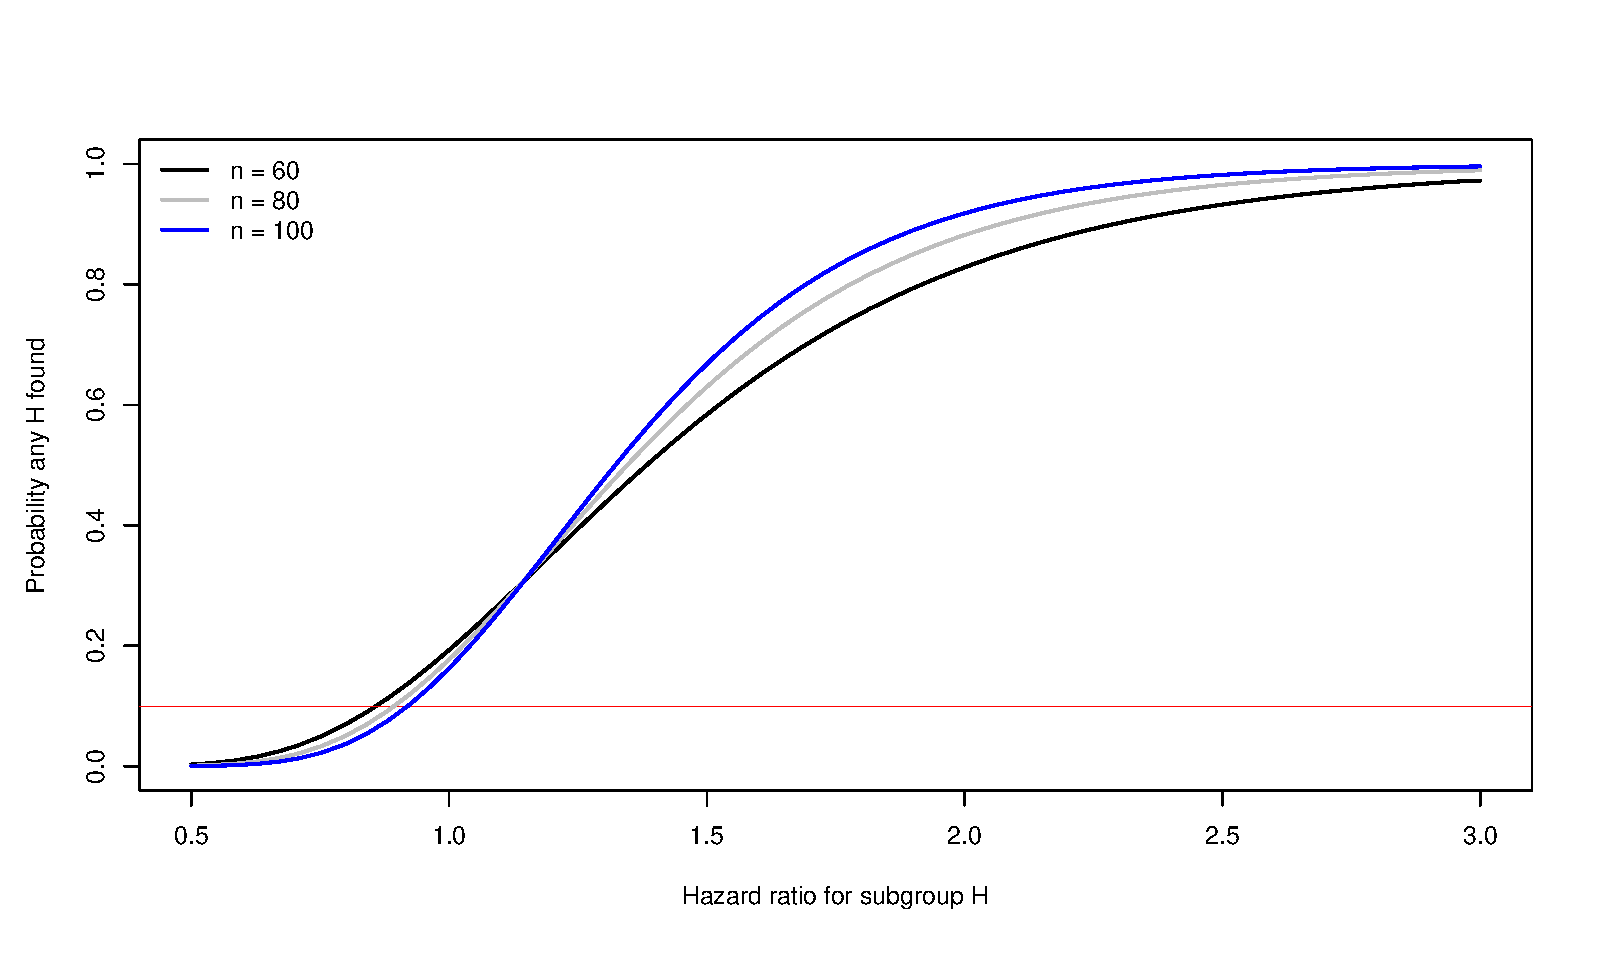
\includegraphics[width=5.5in, height=3.25in]{Figure 2.eps}
\end{center}
\caption{Approximate probability of finding H via FS: Subgroup $H$ of size $n = 60, 80, 100$ with underlying hazard-ratio varying from 0.5 to 3.0 and with average censoring rate of $45\%$ so that $d \approx {0.55}n_{H}$.  The horizontal line indicates $10\%$. Approximately $80\%$ reached at underlying hazard-ratios: $1.94$, $1.81$, and $1.73$, for $n = 60$, $80$, and $100$, respectively. \label{fig:ApproxH}}
\end{figure*}


Figure {\ref{fig:ApproxH}} displays (\ref{pHat_approx}) for scenarios where a subgroup $H$ exists (size $n=$ 60, 80, or 100) with underlying hazard-ratio $\hplim$ ranging from $0.5$ to $3.0$.
Hazard ratios $\leq 1.0$ correspond to non-negative treatment effects and the horizontal line is at $10\%$ suggesting the type-1 error rate is reasonable (with a sharp decline for $\hplim \leq 0.75$).  The power also seems reasonable, generally $\geq 70\%$ for identifying underlying hazard ratios in the $\geq 2.0$ range.  

Our choice of the $1.25$ and $1.0$ thresholds was based on the desire to control the rate for finding a subgroup $H$ to be $\approx 10\%$ when the underlying hazard ratio for $H$ is below 1.0. 
If the underlying treatment effect is uniform and beneficial then for a random subgroup $H$, Cox model estimates will randomly fluctuate around the ITT effect.  For example, for $\hplim \equiv \hplimitt = 0.75$, the above approximation is $0.049$, $0.033$, and $0.022$ (for $n=60$, $80$, and $100$, respectively) indicating reasonable control of type-1 error.  
We note that because FS seeks subgroups with evidence for harm (viz-a-viz the screening and consistency thresholds) the chance of forming subgroups under the null with an estimated benefit randomly in favor of control is less likely the stronger the (uniform) ITT treatment effect.

In Supplementary materials \textcolor{blue}{S1} we provide the power approximations for censoring rates of $0\%$ and $80\%$ (The type-1 error decreases and power increases as the censoring rate decreases.).  In the following simulations we evaluate the type-1 error for falsely identifying a non-existent $H$, and power for subgroup identification under various scenarios designed to mimic potential Phase 2 and Phase 3 trial conditions.








\section{Simulations} \label{sec:sims}

Our simulation setting is based on the German Breast Cancer Study Group trial data (GBSG) \cite{Schumacher_1994,Sauerbrei_1999} that is available in the 
\R{} statistical software survival library.\cite{Rcran,survival-package}  The study sample size was $N=686$ and the outcome of interest 
was tumor recurrence following the addition of hormonal therapy (yes/no) in the adjuvant setting.  The observed censoring rate was $\approx 56\%$ where seven baseline factors were available
including estrogen receptors (fmol/l), age (years), progesterone (prog) receptors (fmol/l), menopausal status (post vs pre), 
number of positive lymph nodes, tumor size (mm), and tumor grade (grade 1/2 vs 3).  We denote these by $W_1$ (\verb+Estrogen+), 
$W_2$ (\verb+Age+), $W_3$ (\verb+Meno+), $W_4$ (\verb+Prog+),  $W_5$ (\verb+Nodes+), $W_6$=(\verb+Size+), 
and $W_7$ (\verb+Grade+), respectively.   

In order to mimic a randomized clinical trial and to have the flexibility to simulate desired sample sizes, we first randomly drew treatment 
arms from the GBSG dataset for a large ``super-population'' of $5,000$ subjects while retaining the subjects' observed covariates.  Specifically, for two synthetic 
treatment arms $2,500$ subjects were randomly drawn with replacement (for each arm) from the $N=686$ subjects to construct a large population that mimics the 
covariate structure of the dataset.  Simulations are then based on randomly sampling from this super-population.  

The outcomes were generated from a Weibull regression model depending on prognostic baseline factors $Z_1-Z_5$ where the $H$ subgroup was generated by a treatment interaction between $Z_1$ (defined below) and $Z_3$, with $Z_3$ denoting post-menopausal status ($Z_3=W_3$). The remaining prognostic factors were $Z_{2} = I(W_{2} \leq \hbox{med}(W_{2}))$, $Z_{4} = I(W_{4} \leq \hbox{med}(W_{4}))$, and $Z_{5} = I(W_{5} \leq \hbox{med}(W_{5}))$.  In addition, $Z_6=W_6$, and $Z_7=W_7$ were observed but non-prognostic, though correlated with $Z_1-Z_5$ per the GBSG dataset.  We defined $k({p_{H}})$ such that for $Z_1=I(W_1 \leq k({p_H}))$, the proportion of subjects in the super-population subgroup with $Z_1=1$ and $Z_3=1$ was $\approx p_{H}$.

The true model was 

\begin{equation}
\log(T)=\mu+\beta_{0}\hbox{V} +  \beta_{1} \hbox{V}Z_{1}Z_{3}  + \beta_2 Z_1 + \beta_3 Z_2 + \beta_4 Z_3 + \beta_5 Z_4 + \beta_6 Z_5 + \tau \epsilon,
\label{dgm0}
\end{equation}


\noindent with $V$ denoting treatment, $\epsilon$ was from the standard extreme value distribution and $\tau$ was a dispersion parameter.  The interaction between $Z_1$ and $Z_3$ represented the subgroup H= $\{Z_{1}=1 \}\cap \{Z_{3}=1\}$ with an underlying proportion of subjects $\approx p_{H}$.  The parameters $\beta_{0}$ and $\beta_{1}$ determined the treatment effects 
where $\beta_{1}=0$ corresponds to no subgroup effect (i.e., $H=\emptyset$). 
For a simulated trial of size $N$, the average number of subjects in the $H$ subgroup was $Np_{H}$ and the average number of subjects in the 
complement $H^{c}$= $\{Z_{1}=0 \}\cup \{Z_{3}=0\}$ was $N(1-p_{H})$.  For example, we considered a scenario with $p_{H} \approx 13\%$ where the size of $H$ was relatively small but practically important and presented a challenge for the identification of $H$ and to the interpretation of an overall (ITT) treatment effect.  

Writing the above data-generating model as 

\begin{equation}
\log(T)=\mu+\beta_{0}\hbox{V}+\beta_{1}\hbox{V}Z_{1}Z_{3}+ {\bm\beta_{2}}'{\bm Z_{2}} + \tau \epsilon, 
\label{dgma}
\end{equation}

\noindent with ${\bm Z_{2}}:= (Z_1, Z_2, Z_3, Z_4, Z_5)$ and ${\bm\beta_{2}}=(\beta_2, \beta_3, \beta_4, \beta_5, \beta_6)$ defined accordingly, we denote the corresponding hazard function when treatment is set to $v$ ($0$ under control; $1$ under treatment) for subjects with given prognostic values (${\bm Z} = {\bm z}$, say) as

\begin{equation}
\lambda_{v}(t;{\bm z})=\lambda_{0}(t)\exp(\gamma_{0}\hbox{v}+\gamma_{1} \hbox{v}z_{1}z_{3}+ {\bm\gamma_{2}}'{\bm z_{2}}),
\label{dgmh}
\end{equation}

\noindent where $\gamma = - \tau \beta$, \cite{ACR_2015} say.  The parameters $\mu$, ${\bm\beta_{2}}$, and $\tau$ were based on Weibull model fits to the observed GBSG data with $\beta_0$ and $\beta_1$ then chosen to generate (marginal) hazard ratio subgroup effects of interest in the ``super-population'' (e.g., $\hplim=2.0$, and $\hcplim =0.65$).  

A covariate-dependent censoring distribution was also generated by a Weibull model analogous to (\ref{dgma}) based on the observed data in order to have a censoring rate of approximately $46\%$ (however here there is no subgroup effect, $\beta_{1} \equiv 0$).

We evaluate the operating characteristics for identifying and estimating $H$ and $H^{c}$ under various sample sizes and treatment effects.  Under the null model with $\beta_{1}=0$ ($H=\emptyset$), $H^{c}$ is the ITT population with (marginal) hazard ratio $\hplimitt$. We note that for fixed $p_{H}$ as $\beta_{1} \neq 0$ varies, inducing subgroup effect $\hplim$, the overall (ITT) population effect $\hplimitt$ will also vary; 
whereas the complementary subgroup effect $\hcplim$ will remain constant.  

For identification and estimation we are targeting marginal hazard ratios for $H$ and $H^{c}$ in the super-population where subgroup analyses are based on Cox models that solely adjust for treatment.  That is, 
excepting for treatment assignment Cox model analyses are un-adjusted for covariates.   As described by Aalen et al\cite{ACR_2015} the marginal effects for $H$ and $H^{c}$ will generally differ from  their {\it controlled direct effects} which we denote by $\hhplim$ and $\hhcplim$.  From (\ref{dgmh}) note that $\hhplim = \exp(\gamma_{0}+\gamma_{1})$, and $\hhcplim = \exp(\gamma_{0})$.   When describing FS estimation properties in Section \ref{sec:boot} we will consider accuracy in terms of both $\theta^{\dagger}(.)$ and $\theta^{\ddagger}(\cdot)$.

Now, in addition to the proposed FS approach we evaluate virtual twins\cite{FTR_2011} and GRF\cite{ATW_2019,AW_2021,CZ_2023} procedures for subgroup identification.  
To account for censoring with the virtual twins approach we employ a basic ``censoring unbiased transformation''\cite{FG_2018} (Doubly-robust versions are also available\cite{SDS_2019}).  Virtual twins is implemented via the \R{} package \verb+aVirtualTwins+,\cite{vtR} and generalized random forests is implemented using the \verb+causal_survival_forest+ function in the \R{} \verb+grf+ package.\cite{grfR,SAW_2023}  When utilized in the FS algorithm lasso is implemented with the \verb+glmnet+ \R{} package.\cite{SFHT_2011}  

For GRF and virtual twins we restrict to subgroups where sample sizes are at least $60$ subjects and to a maximum tree depth of 2; subgroups are selected as follows.

\begin{enumerate}[{GRF:}]
\item{GRF targets RMST and we denote GRF as RMST based on the truncation point $\tau=\min(\tau_{0},\tau_{1})$ where $\tau_{0}$ and $\tau_1$ are the largest non-censored (event) outcomes for the control and treatment groups (respectively).
An estimated RMST benefit of (at least) $6$ months for control is required for selection of a subgroup $H$, where among tree depths of 1 and 2, the subgroup with the largest RMST benefit ($\geq 6$ months) in favor of control is selected.}
\end{enumerate}
\begin{enumerate}[{GRF.60:}]
\item{The GRF procedure employs a double-robust approach for estimating RMST that involves estimation of the censoring distribution.  As such, the choice of the truncation point can be influential.  To reduce the potential instability we consider GRF.60 which uses $\tau_{60}:= 0.6\min(\tau_{0},\tau_{1})$.}
\end{enumerate}
\begin{enumerate}[{VT(24):}]
\item{We consider the virtual twins approach targeting survival rates at $t=24$ months. A treatment effect of $\delta \geq 0.225$, in favor of control, is required for selection of $H$.}
\end{enumerate}
\begin{enumerate}[{VT(36):}]
\item{Same as $\hbox{VT(24)}$ but with $t=36$.}
\end{enumerate}

To quantify the classification properties we consider the following sensitivity and positive predictive value measures.  For 
estimated subgroup $\widehat{H}$ define ${sens}(\widehat{H})$ and ${ppv}(\widehat{H})$ as

\begin{equation}
{sens}(\widehat{H}) = \# \{i \in \widehat{H} \cap H \} / \# \{i \in H \}, \ \hbox{and} \ {ppv}(\widehat{H}) = \# \{i \in \widehat{H} \cap H \} / \# \{i \in \widehat{H} \},
\nonumber
\end{equation}
\noindent
with measures for the complement $\widehat{H}^{c}$ defined analogously. Note that there always exists ${\widehat H}^{c}$ for any procedure, since if a candidate subgroup does not meet the criteria of a procedure then $\widehat H = \emptyset$ 
and the estimated complement is set to the overall ITT population (${\widehat H}^{c}= \Omega$, say).  Under the null when no 
subgroup $H$ exists, the denominator in $sens(\widehat{H})$ is zero and the numerator in $ppv(\widehat{H})$ is zero, thus $sens(\widehat{H})$ is undefined and $ppv(\widehat{H}) \equiv 0$.


\subsection{Chance of finding any subgroup $H$} \label{sec:simsA}

In our simulation study we consider three data generation models, denoted $M_1, M_2$, and $M_3$, where performance of the methods were evaluated under null and alternative subgroup effect conditions across $20,000$ simulations.   Under each model scenario we consider the performance when the clinical factors $Z_{1}-Z_{7}$ are evaluated as well as when additional (completely random) noise factors are artificially included (e.g., $Z_{8}, Z_{9},$ and $Z_{10}$ are each independent standard normal random variables). Recall $Z_1-Z_5$ are truly prognostic ($Z_6$ and $Z_7$ are non-prognostic but correlated with the others) and the underlying subgroup is $H= \{Z_1=1 \} \cap \{Z_3=1 \}$.

Table \ref{tab:m4} displays the probabilities for identifying a subgroup $H$, denoted $any(H)$, as well as the classification rates for each analysis approach under the null ($H= \emptyset$) and alternative.  Under 
the alternative the (marginal) hazard ratio for the subgroup $H$ was $\theta^{\dagger}(H)=2.0$ for each model $M_1-M_3$.  Under the null, we consider rates above $10\%$ for falsely identifying a subgroup $H$ (type-1 error) as generally inflated; approaches where $any(H) \geq 0.10$ are bold-faced in the table.  

For model $M_1$, the first block, there were $N=700$ subjects where under the null ($H = \emptyset$, denoted ``$M_{1}$ Null'') and alternative (denoted ``$M_{1}$ alt'') the hazard ratios for the ITT population, $\theta^{\dagger}(ITT)$, were similar at $0.7$, and $0.71$, respectively. Under the alternative the proportion of subjects in the true $H$ subgroup was $p_{H} \approx 13\%$ and the hazard ratio for $H^{c}$ was $\theta^{\dagger}(H^{c})= 0.65$.   In the scenario when only real clinical factors $Z_1, \ldots, Z_7$ were included in the analysis (The first 6 columns), under the null, all 
of the approaches controlled the type-1 error at $\leq 5\%$ except $\grfa$ which was at 
$25\%$.  Under the alternative, $\fsl$ and $\fslg$ both outperform $\grfb$ (and virtual twins) with higher rates for identifying $H$ and classification accuracy. For example, for $\fslg$ the chance of identifying any $H$ was $86\%$ and the accuracy for correctly classifying subjects in $H$, $sens(\widehat{H})$, was $82\%$; whereas for $\grfb$ these rates were $72\%$ and 
$66\%$, respectively.   When the analysis included three additional random noise factors, columns 7-12, the type-1 error rates for the GRF approaches were both quite elevated ($61\%$, and $27\%$ for $\grfa$ and $\grfb$, resp.)  with 
$\fslg$ slightly elevated at $11\%$ whereas $\fsl$ was at $2\%$.  Moreover, despite the higher type-1 error for $\grfb$, $\fsl$ and $\fslg$ both had higher classification accuracy (e.g., $sens(\widehat{H})$ was $64\%$ [$74\%$] for $\fsl$ [$\fslg$] compared to $52\%$ for $\grfb$).

A similar pattern to model $M_1$ is found under $M_2$ where we consider a smaller sample size but with a higher proportion of subjects in the $H$ subgroup.  Specifically, 
model $M_2$ had $N=500$ subjects where under the null and alternative $\theta^{\dagger}(ITT)$ was $0.69$ and $0.79$ (resp.), $p_{H} \approx 20\%$ and $\theta^{\dagger}(H^{c})= 0.69$.   In addition, we consider the performance when five additional random noise factors were included in the analysis.  The type-1 errors were similar to model $M_1$, however the identification and accuracy rates were higher for $H$ relative to model $M_1$ even though the incidence rate for $H$ was only moderately increased (The average size for $H$ under models $M_1$ and $M_2$ were $89$ and $101$, resp.).

Lastly, we consider a relatively smaller sample size of $N=300$ in model $M_3$ with a stronger ITT treatment effect under the null where $\theta^{\dagger}(ITT) = 0.55$.  In this scenario all the 
approaches controlled the type-1 error rates below $5\%$ except for $\grfa$ and $\grfb$ which were slightly elevated ($13\%$, and $7\%$, resp.) when five additional random noise factors were included in the analysis.  In this scenario $\grfa$ had the strongest performance, albeit with the aforementioned increased type-1 error rate, whereas $\fslg$ had the highest accuracy while maintaining the type-1 error at $\leq 2\%$.

We note that while the accuracy for classification of $H^{c}$ subjects via $sens(\widehat{H}^{c})$ remains seemingly high in the presence of additional noise factors ($\geq 87\%$), the $\fslg$ approach was around $7\%$ higher compared to $\grfb$ for some scenarios (e.g., $96\%$ vs. $89\%$ under the $M_2$ alternative).  Though not dramatic, this could be important in clinical practice from an individual patients' perspective.

In this simulation setting when random noise factors were included in the analyses the GRF approach was more susceptible to falsely identifying subgroups especially under models $M_1$ and $M_2$.  Intuitively, with the addition of noise factors there was more opportunity to randomly form erroneous splits.  For virtual twins, the type-1 errors were not materially increased but the accuracy performance was 
generally diluted across the scenarios.  The $\fsl$ approach was the most stable with a slight decrease in performance, while $\fslg$ inherits an increased type-1 error by the utilization of $\grfb$, but to a much lesser extent than $\grfb$ itself.  In contrast, under $M_3$ when there was the strongest ITT treatment effect under the null, the type-1 errors for both GRF approaches were dramatically decreased relative to $M_1$ and $M_2$ (From $\approx 60\%$[$30\%$] for $\grfa$[$\grfb$] under $M_1$ and $M_2$ to $13\%$[$7\%$] under $M_3$.).  We conjecture that this is due to the GRF selection criteria which requires an estimated 6-month benefit in favor of control, which is less likely with a more pronounced ITT treatment effect (Note that under the nulls of $M_1-M_3$ the ITT treatment differences with respect to RMST were $\approx$ $7.2$, $7.4$, and $11.5$ months, resp.).  Generally, for each approach under the null, the chance of forming subgroups with an estimated benefit randomly in favor of control is less likely the stronger the ITT treatment effect.  Table \ref{tab:m4} also provides the approximation (\ref{pHat_approx}) to the power for the FS procedure (see footnotes a-f) which appears reasonably accurate for models $M_1 - M_3$.




















\subsection{FS bootstrap bias-correction and variance estimation} \label{sec:boot}

By the nature of the FS procedure we expect un-adjusted Cox model estimates based on $\widehat{H}$ to be upwardly biased due to the hazard ratio thresholds, especially for $\hplim \leq 1.25$ (Since by construction point estimates are $\geq 1.25$ for $\widehat{H}$). However the bias can also be pressured in the opposite direction depending on the proportion of $H^{c}$ subjects (incorrectly) included in $\widehat{H}$ and the value of $\hplim$ relative to $\hcplim$ (e.g., mixture of $\hplim=2.0$ vs. $\hcplim=0.65$).  In general there is potential for exacerbating estimation bias due to the subgroup selection.  For bias-correction, we proceed on the Cox regression coefficient scale, denoted $\hat\beta(\widehat{H})$, and then exponentiate to obtain point estimates and confidence intervals for hazard ratios $\hat\theta(\widehat{H}):= \exp(\hat\beta(\widehat{H}))$.

Our bias corrected estimator takes into account two sources of bias which involve the discrepancies between the bootstrapped and observed data Cox estimators, $\hat\beta^{*}_{b}(\cdot) - \hat\beta(\cdot)$ say, evaluated separately at the bootstrapped and observed subgroup estimates.   The bias corrected estimator $\hat\beta^{*}(\widehat{H})$ described below is along the lines of  Harrell et al.\cite{Harrell_1996}  However our understanding is that the latter\cite{Harrell_1996} does not involve the bias term involving $\hat\beta^{*}_{b}(\widehat{H}) - \hat\beta(\widehat{H})$.   

For the observed data with estimated subgroup $\widehat{H}$ define $\hat\beta(\widehat{H})$ as the estimated Cox model regression parameter.  Analogously, for 
bootstrap samples $b=1,\ldots,B$ with estimated subgroup $\widehat{H}^{*}_{b}$, let $\hat\beta^{*}_{b}(\widehat{H}^{*}_{b})$ 
denote the estimated Cox model parameter for the bootstrap sample based on subgroup $\widehat{H}^{*}_{b}$.  In addition, 
let $\hat\beta(\widehat{H}^{*}_{b})$ denote the Cox model parameter for the observed data based on the bootstrap estimated subgroup $\widehat{H}^{*}_{b}$ (That is, the Cox model estimate applied to the observed data within the subgroup defined by $\widehat{H}^{*}_{b}$.). 
Define $\hat\beta^{*}_{b}(\widehat{H})$ similarly and form the bias terms $\eta_{b}^{*}(\widehat{H}^{*}_{b})= \hat\beta^{*}_{b}(\widehat{H}^{*}_{b}) - \hat\beta(\widehat{H}^{*}_{b})$ and $\eta_{b}^{*}(\widehat{H})= \hat\beta^{*}_{b}(\widehat{H}) - \hat\beta(\widehat{H})$
for $\hat\beta(\widehat{H})$.  Correspondingly, for the complementary subgroup, define $\eta_{b}^{*}(\widehat{H}^{c*}_{b})$ and $\eta_{b}^{*}(\widehat{H}^{c})$ for $\hat\beta(\widehat{H}^{c})$ analogously.  Let $\{(\eta_{b}^{*}(\widehat{H}^{*}_{b})+\eta_{b}^{*}(\widehat{H})), (\eta_{b}^{*}(\widehat{H}^{c*}_{b}) + \eta_{b}^{*}(\widehat{H}^{c}))\}$ denote bootstrap samples $b=1,\ldots,B$.
The bias-corrected estimators are defined as 

\begin{equation}
\hat\beta^{*}(\widehat{H})=\hat\beta(\widehat{H})-(1/B)\sum_{b=1}^{B} (\eta_{b}^{*}(\widehat{H}^{*}_{b}) + \eta_{b}^{*}(\widehat{H})), \quad \hat\theta^{*}(\widehat{H}) = \exp(\hat\beta^{*}(\widehat{H})),
\label{Hboot_bc}
\end{equation}

\begin{equation}
\hat\beta^{*}(\widehat{H}^{c})=\hat\beta(\widehat{H}^{c})-(1/B)\sum_{b=1}^{B} (\eta_{b}^{*}(\widehat{H}^{c*}_{b}) + \eta_{b}^{*}(\widehat{H}^{c})), \quad \hat\theta^{*}(\widehat{H}^{c}) = \exp(\hat\beta^{*}(\widehat{H}^{c})).
\label{Hcboot_bc}
\end{equation}

\noindent
The bootstrap samples are drawn independently with replacement from the observed data $\{O_{i}:=(V_{i},Z_{i},Y_{i},\Delta_{i}),$ $i=1,\ldots,N \}$.   To estimate the variance we apply an infinitesimal jacknife approximation\cite{Efron_2014,Wager_2014} viewing (\ref{Hboot_bc}) and (\ref{Hcboot_bc}) as ``bagged estimators'' which has been utilized in related contexts.\cite{Rosenkranz_2016,Ballarini_2021}  

We describe the variance estimation for $\hat\beta^{*}(\widehat{H})$ given by (\ref{Hboot_bc}); the variance for the complement (\ref{Hcboot_bc}) is completely analogous.  Let $O^{*}_{b} = \{O^{*}_{b1},O^{*}_{b2},\ldots,O^{*}_{bN} \}$ denote bootstrap sample $b=1,\ldots,B$ which we write as $\{O^{*}_{bj}, j=1,\ldots,N \}$.  Let $K^{*}_{bi}=\# \{O^{*}_{bj}=O_{i}  \}$ 
denote the number of times the $i$'th observation $O_{i}$ is drawn for the $b$'th bootstrap sample, and let $\bar{K}^{*}_{i}=(1/B)\sum_{b=1}^{B}K^{*}_{bi}$.  The intinitesimal jacknife variance estimate for $\hat\beta^{*}(\widehat{H})$ is given by

\begin{equation}
\tilde{V} = \sum_{i=1}^{N} \widetilde{cov}_{i}^{2}, \quad \widetilde{cov}_{i}=(1/B)
\sum_{b=1}^{B}(K^{*}_{bi}-\bar{K}^{*}_{i})\big(\hat\beta(\widehat{H})-\eta_{b}^{*}(\widehat{H}^{*}_{b})- \eta_{b}^{*}(\widehat{H}) -\hat\beta^{*}(\widehat{H})\big),
\label{VInfJ}
\nonumber
\end{equation}

\noindent
with bias-corrected version $\hat{V}$\cite{Wager_2014} given by 

\begin{equation}
\hat{V} := \tilde{V} - \frac{N}{B} \tilde\sigma^{2}_{B}, \quad \tilde\sigma^{2}_{B}=(1/B)\sum_{b=1}^{B}\big(\hat\beta(\widehat{H})-\eta_{b}^{*}(\widehat{H}^{*}_{b}) - \eta_{b}^{*}(\widehat{H}) -\hat\beta^{*}(\widehat{H}) \big)^{2}.
\label{VInfJ_bc}
\end{equation}

In this work, the variance estimate for the bias-corrected parameter estimator will be given by $\hat{V}$ in (\ref{VInfJ_bc}) and $95\%$ confidence intervals for hazard ratios, 
$\hat\theta^{*}(\widehat{H})$ and $\hat\theta^{*}(\widehat{H}^{c})$ defined in (\ref{Hboot_bc}) and (\ref{Hcboot_bc}) respectively, will be based on standard normal approximations (exponentiated).  
For the $\fsl$ and $\fslg$ estimators the lasso and $\grfb$ algorithms are mimicked for the bootstrap versions.  In general, the variance induced by the (well-defined) candidate selection algorithm is incorporated by mimicking the algorithm in the bootstrap process.



For summarizing estimation properties we consider bias with respect to three targets described below.   Recall, the hazard function for subjects with covariate vector characteristics ${\bm Z}={\bm z}$ with treatment set to $v$ ($0$ under control, $1$ under treatment) is given by 
$\lambda_{v}(t;{\bm z})=\lambda_{0}(t)\exp(\gamma_{0}\hbox{v}+\gamma_{1} \hbox{v}z_{1}z_{3}+ {\bm\gamma_{2}}'{\bm z_{2}}),$
and define $\theta_{v}(t) = E_{{\bm Z}}{\lambda_{v}(t;{\bm Z})}$ with the expectation over the joint covariate distribution.  We define 
the {\it controlled direct effect (CDE)} of treatment as $\theta^{\ddagger} = \theta_{1}(t)/\theta_{0}(t)$,\cite{ACR_2015} and for a generic subgroup $G$, $\theta^{\ddagger}(G)$ is defined with 
the expectation restricted to $G$ (e.g., if $G$ is defined by $\{Z_{1} = 1 \} \cap \{ Z_{4}=1 \}$).    In particular, for the true subgroups $H$ and $H^{c}$, 

\begin{equation}
\theta^{\ddagger}(H) = \exp(\gamma_{0}+\gamma_{1}), \quad \hbox{and} \quad 
\theta^{\ddagger}(H^{c}) = \exp(\gamma_{0}).  
\nonumber
\end{equation}

\noindent
For estimated subgroups which will generally consist of a mixture of subjects from $H$ and $H^{c}$ we 
use the empirical sample version of the above expectations.  That is, for subjects in $\widehat{H}$ let 
$\bar\theta_{v}(t;\widehat{H}) =\lambda_{0}(t) \exp(\gamma_{0}v) \sum_{i \in \widehat{H}} \exp(\gamma_{1}\hbox{v}z_{i,1}z_{i,3}+ {\bm\gamma_{2}}'{\bm z_{i,2}})$ and define

\begin{equation}
\theta^{\ddagger}(\widehat{H}) = \bar\theta_{1}(t;\widehat{H}) / \bar\theta_{0}(t;\widehat{H}) = \exp(\gamma_{0})\frac{\sum_{i \in \widehat{H}} \exp(\gamma_{1}z_{i,1}z_{i,3}+ {\bm\gamma_{2}}'{\bm z_{i,2}})}
{\sum_{i \in \widehat{H}} \exp({\bm\gamma_{2}}'{\bm z_{i,2}})},
\label{cdeH}
\end{equation}

\noindent where recall for subjects in $H$, $z_{i,1}z_{i,3} \equiv 1$ so the above reduces to $\theta^{\ddagger}(H)$ if $\widehat{H} \equiv H$ ($\widehat{H}$ consists only of subjects in $H$).   
Similarly, define $\theta^{\ddagger}(\widehat{H}^{c})$ with $\widehat{H}$ substituted with $\widehat{H}^{c}$ in equation (\ref{cdeH}). 

Recall that for each simulated dataset the $\gamma$ parameters are (known and) fixed for each model $M_1 - M_3$, however the covariates are randomly drawn from the ``super-population''.  Therefore, 
even for two simulated datasets with the same definition of $\widehat{H} \neq H$, for example $\{Z_{1} = 1 \} \cap \{ Z_{4}=1 \}$, the $\theta^{\ddagger}(\widehat{H})$ quantities will vary for each simulated dataset due to variation in the other covariates.  The CDE's $\theta^{\ddagger}(\widehat{H})$ and $\theta^{\ddagger}(\widehat{H}^{c})$
are thus random quantities with respect to $\widehat{H}$ and the covariates.

We evaluate bias and $95\%$ CI coverage properties for the $\fslg$ estimator, as well as the oracle estimator (i.e., under the ideal scenario where the true $H$ and $H^{c}$ subgroups are known a-priori).  Let $\hknow$ denote the oracle Cox estimator, with $\hhat$ and $\hhatB$ the observed and bootstrap bias-corrected versions based on the $\fslg$ procedure, respectively.  
For each estimator $\hat\theta(H)$, $\hhat$, and $\hhatB$, we consider three targets: $\hknow$, $\theta^{\ddagger}(\widehat{H})$, and $\theta^{\dagger}(H)$.  For each estimator define 
the $\%$ relative biases: $\hat{b}^{oracle}$, $\hat{b}^{\ddagger}$, and $b^{\dagger}$ which are relative to $\hknow$, $\theta^{\ddagger}(\widehat{H})$, and $\theta^{\dagger}(H)$, respectively.  For example, for $\hhat$: $\hat{b}^{oracle} = (\hhat - \hknow)/\hknow$, 
$\hat{b}^{\ddagger} = (\hhat - \Hhplim)/ \Hhplim$, and $b^{\dagger} = (\hhat - \hplim)/\hplim$, which are multiplied by $100$ to represent $\%$ relative bias.  Define corresponding coverage measures as $\hat{C}^{oracle}$, $\hat{C}^{\ddagger}$, and $C^{\dagger}$ 
to indicate whether the $95\%$ confidence interval covers the respective target.  For example, for  $\hhatB$, $\hat{C}^{\ddagger}$ is the proportion of times the $95\%$ CI for $\hhatB$ includes (the random) $\theta^{\ddagger}(\widehat{H})$.  

Table \ref{tab:m1B-m3B} summarizes the properties of the $\fslg$ estimator under models $M_1 - M_3$ when additional noise factors are included.  Summaries are based on estimable (evaluable) realizations (across $1,000$ simulations and $B=300$ bootstraps) where $\{\hhatB, \hchatB \}$ exists. 

For the observed $\hhat$ the (average) relative bias, $b^{\dagger}$ [$\hat{b}^{\ddagger}$] ranged from approximately $9.2\%$ to $24\%$ [$9.0\%$ to $14\%$] across the $M_1 - M_3$ models; indicating a general over-estimation for Cox hazard ratios based on estimated subgroups.  In contrast, for the bias-corrected $\hhatB$,  $b^{\dagger}$ [$\hat{b}^{\ddagger}$] ranged from $-10\%$ to  $-2.4\%$ [$-11.60\%$ to $- 6.3\%$]. 
For $\hchat$, $b^{\dagger}$ [$\hat{b}^{\ddagger}$] ranged from $0.5\%$ to $5.1\%$ [$-9.7\%$ to $2.8\%$], and for $\hchatB$,  $b^{\dagger}$ [$\hat{b}^{\ddagger}$] ranged from $2.3\%$ to  $10.9\%$ [$-4.8\%$ to $4.6\%$]. 

For standard deviation and CI accuracy we summarize the results for $\hchatB$ under model $M_3$ which has the highest difference between $\hcplim = 0.56$ and $\hhcplim=0.49$.  Here the standard deviations for $\hchat$ 
are under-estimated ($0.13$ for the empirical SD's versus $0.11$ for the average of the estimated SD's) with (slight) under-coverage for $\hcplim$ ($C^{\dagger}=92\%$) and under-coverage for $\Hhcplim$ ($\hat{C}^{\ddagger}=76\%$).  In contrast, the standard deviations for $\hchatB$ are over-estimated ($0.14$ versus $0.17$) with coverage rates $C^{\dagger}=97\%$ and $\hat{C}^{\ddagger}=93\%$.

In this setting, under models $M_1 - M_3$, the bootstrap bias-corrected estimators tend to be conservative: Under-estimating both $\hplim$ and $\Hhplim$ (``conservative for harm'') while over-estimating both $\hcplim$ and $\Hhcplim$ (``conservative for benefit''), except for under model $M_3$ where $\hat{b}^{\ddagger} \approx -4.8 \%$.  In addition, the coverage rates for $\hchatB$ are $\geq 93\%$ for each target, and the oracle coverage rates ($\hat{C}^{oracle}$) for the observed and bias-corrected estimators are $\geq 95\%$. That is, the observed and bias-corrected versions of $\widehat{H}$ and $\widehat{H}^{c}$ cover ($\geq 95\%$) their respective oracle counterparts.

\section{Applications} \label{sec:applications}

In applications, as suggested by a reviewer, we consider cross-validation (CV) for evaluating the 
quality and stability of the selection algorithms (See also Athey and Wager\cite{AW_2021}, and Knaus\cite{Knaus_2022}).  
Two forms of CV are implemented, 10-fold CV, and what we refer to as $N$-fold CV defined as follows.   For $N$-fold CV we 
exclude each subject ($i=1,\ldots,N$) from the analysis and predict their $\widehat{H}$ ($\widehat{H}^{c}$) classification (based on the remaining $N-1$ subjects) where if 
a subgroup $\widehat{H}$ is not identified then the subject is classified as $\widehat{H}^{c}$ (i.e., $\widehat{H}= \emptyset$).   That is, let $\hat\pi^{-i}({\bm Z}_{i})$ denote 
the $i$th subjects' predicted 
classification based on the FS procedure ($\widehat{H}$ or $\widehat{H}^{c}$) without the subject in the analysis.  Similarly define  $\hat\pi({\bm Z}_{i})$ 
as the FS classification based on the full sample analysis and form $\widehat{O}_{CV}=\{\hat{O}_{i}:=(V_{i},Y_{i},\Delta_{i},\hat\pi({\bm Z}_{i}),
\hat\pi^{-i}({\bm Z}_{i})),$ $i=1,\ldots,N \}$.  Cox model analyses based on $\hat\pi(\cdot)$ subgroups correspond to estimates that are un-adjusted for the selection algorithm 
whereas $\hat\pi^{-i}(\cdot)$ represents an {\it out-of-bag (OOB)} classification where each subject is not included in the selection algorithm from which they are classified.  Correspondence between $\hat\pi(\cdot)$ and $\hat\pi^{-i}(\cdot)$ subgroup analysis results may be anticipated, especially for large $N$.  Of course if $\hat\pi$ and $\hat\pi^{-i}$ are identical then there is no diagnostic value; in contrast substantial lack of correspondence may suggest an underlying instability.  In 10-fold CV we randomly partition the data into 10 folds and for each fold (leaving these subjects out) select $\widehat{H}$ based on the other 9 folds to predict the classification for that left out fold. This yields an alternative version of $\widehat{O}_{CV}$ where $\hat\pi^{-i}$ now corresponds to the predicted classification based on the left out fold analysis to which the $i$th subject belongs.  Since this process generally depends on the random partition we repeat this $200$ times and summarize correspondence measures across the partitions. 

For both CV approaches we consider metrics such as how often a subgroup is identified based on the ``training samples'' and the correspondence with the full sample analysis $\widehat{H}$ definitions, as well as in terms of sensitivity and positive predictive value measures.  To this end, the sensitivity and positive predictive value  metrics in Section \ref{sec:sims} are modified by replacing $\widehat{H}$ with $\widehat{H}^{-i}$ (i.e., $\hat\pi^{-i}$) and the true $H$ with $\widehat{H}$. For example, ${sensCV}(\widehat{H}): = \# \{i \in \widehat{H}^{-i} \cap \widehat{H} \} / \# \{i \in \widehat{H} \}$ denotes the correspondence between the CV ``testing prediction'' and the full analysis $\widehat{H}$-classification (relative to the size of the full analysis $\widehat{H}$).

In the sequel, for a generic baseline factor $Z$ we denote the binary split at $a$ by \verb+Z<=a+ to represent the baseline factor candidate $X = I(Z \leq a)$ which would correspond to candidate subgroup indicators $J=\{Z \leq a\}$ and $J^{c} = \{Z > a \}$ (say).






  

  
  

  
  
  


\begin{figure}
\begin{center}
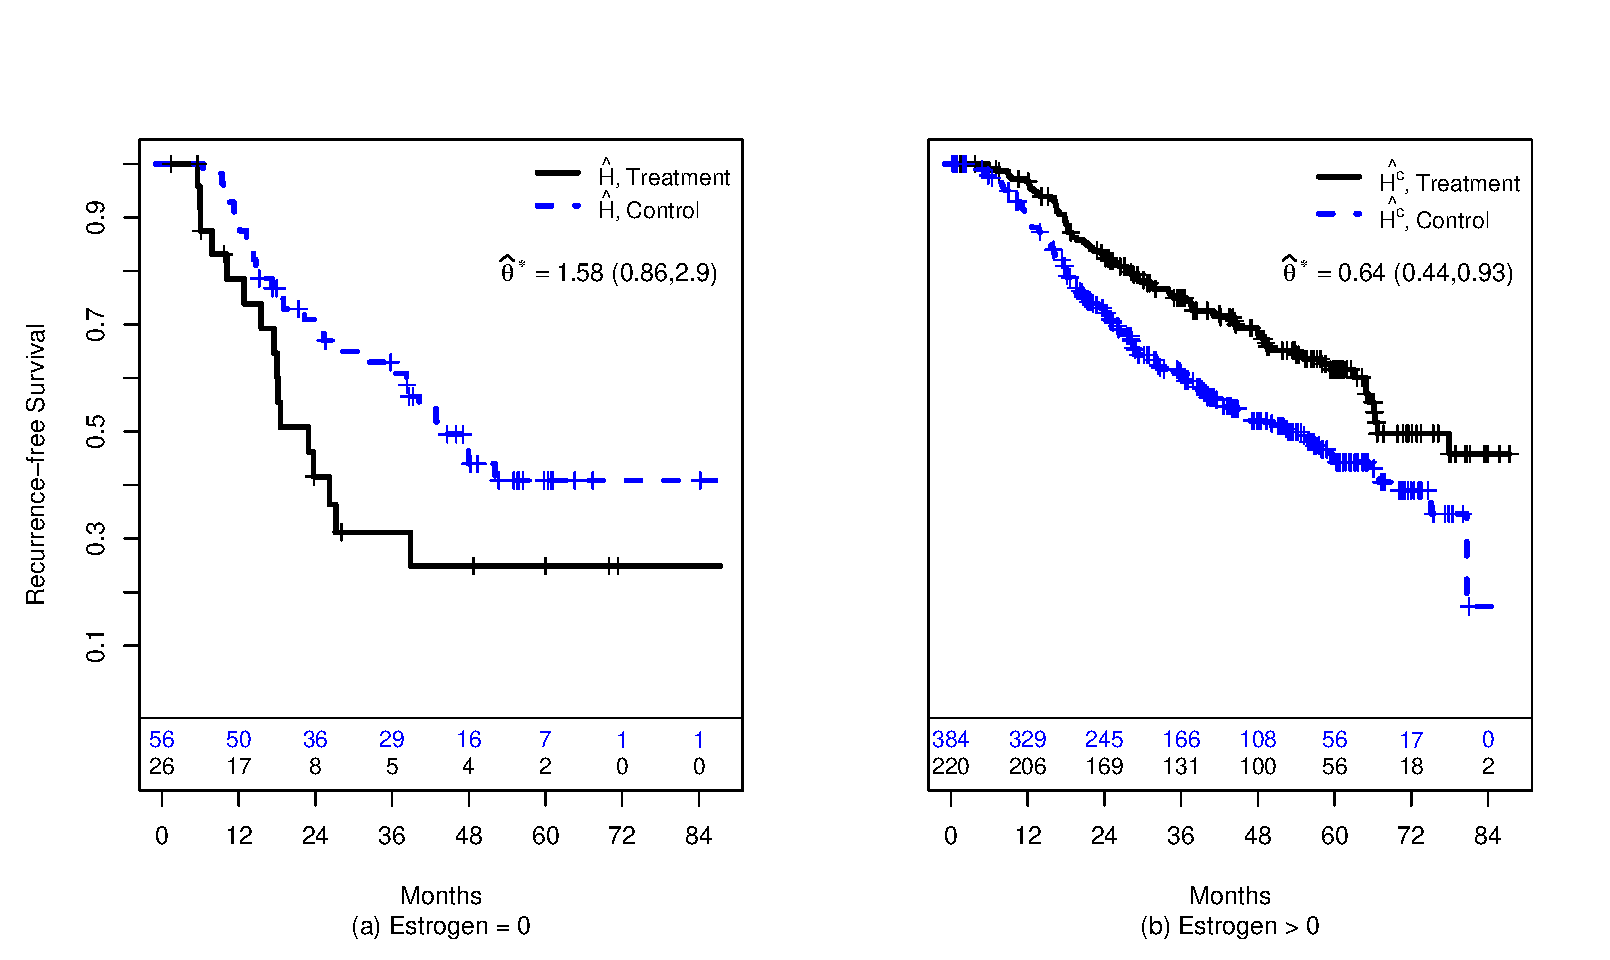
\includegraphics[width=\textwidth, height=3.25in]{Figure 3.eps}
\end{center}
\caption{GBSG analysis application of Forest Search. Kaplan-Meier (K-M) curves (un-adjusted for the estimation of subgroups) with bootstrap-bias corrected 
Cox estimates and $95\%$ confidence intervals denoted $\hat\theta^{*}$: (a) Forest Search $\widehat{H}$ subgroup; (b) Forest Search $\widehat{H}^{c}$ subgroup.}
\label{fig:gbsg}
\end{figure}


\subsection{GBSG analysis}

In our first application we return to the breast cancer study\cite{Schumacher_1994,Sauerbrei_1999} described in Section \ref{sec:sims}.  Recall the study sample size was $N=686$ where 
we consider the comparison of tamoxifen (hormonal) treatment to chemotherapy.  The observed censoring rate was $\approx 56\%$, and the Cox ITT hazard ratio estimate ($95\%$ CI) was $0.69$ ($0.54$, $0.89$). There were $p=7$ prognostic factors collected: \verb+Estrogen+, \verb+Age+, \verb+Prog+, \verb+Meno+, \verb+Nodes+, \verb+Size+, and \verb+Grade+.   The factors \verb+Meno+ and \verb+Grade+ (grade 1/2 vs 3) are categorical and the rest are continuous. 

In this analysis we select the largest subgroup with a consistency rate of at least $90\%$ where lasso\cite{SFHT_2011} is first applied with the aforementioned factors, and for the continuous factors (selected per lasso), these are cut at the mean, median, 1st quartile, and 3rd quartile.  We note that an alternative analysis where lasso is not applied yields the same estimated subgroups and virtually identical bootstrap bias-corrected estimates (described below).  In addition, another alternative analysis maximizing the consistency rate is described in Supplementary materials \textcolor{blue}{S2.1}.  In comparison to these alternative analyses, the 10-fold CV properties for the current analysis suggests preferable algorithmic stability (details described below).  

Now, the first stage of our algorithm is to apply lasso which selects \verb+Grade+, \verb+Size+,  \verb+Nodes+, and \verb+Prog+, the last 
three of which are continuous, and binary cuts at the mean, median, 1st quartile, and 3rd quartile were included for each continuous factor. Next, applying GRF ($\grfb$ with a 6-month RMST criterion) selects \verb+Estrogen<=0+ (Estrogen cut at $0$).  There were then $K=14$ candidate factors (binary cuts) and thus $L = 28$ total single factor subgroups with $L(L-1)/2+L = 406$ possible subgroups (two-factor combinations); among these subgroups the number of candidates with sample sizes $\geq 60$ and at least $10$ events in each arm was reduced to $263$. 

The FS approach estimates $\widehat{H}$ as the subgroup \verb+Estrogen<=0+ (The consistency rate is $95.1\%$).  That is, $\widehat{H}$ subjects are those with an estrogen level of $0$ and the resulting $\hat{H}$-estimates were $\hhat = 1.95$ ($1.05$, $3.61$) with bootstrap bias-corrected $\hhatB =1.58$ ($0.86$, $2.9$).  For the complement, $\hchat = 0.61$ ($0.47$, $0.8$) and $\hchatB =0.64$ ($0.44$, $0.93$).  The bias-corrected estimate for $H^{c}$ suggests a slightly stronger benefit ($0.64$ vs $0.69$ for ITT) that is statistically significant and corresponds to $604/686 \approx 88\%$ of the ITT population.   Whereas for $H$, the bias-corrected estimate is not statistically significant for detriment but may suggest careful consideration for subjects without positive estrogen levels. Figure \ref{fig:gbsg} displays the Kaplan-Meier curves for the estimated subgroups.

For $N$-fold CV, across the $N=686$ training sets (based on deleting a single subject) 
all analyses identified \verb+Estrogen<=0+.  Therefore, the $N$-fold $\hat\pi^{-i}(\cdot)$ and observed (un-adjusted) 
$\hat\pi(\cdot)$ are identical (i.e., no actual adjustment via $N$-fold CV).  In contrast, across the $200$ random 10-fold CV analyses the median number of training sets (10 folds) with an identified subgroup was 9 out of 10 (The minimum was 5/10 with lower and upper quartiles of 8/10 and 9/10, resp.) resulting in a sensitivity of $sensCV(\widehat{H}) = 73\%$.  That is, among the $\widehat{H}$-classified subjects based on the full analysis the median percentage also $\widehat{H}$-classified in the (10-fold) CV testing samples was approximately $73\%$. The median positive predictive value was $ppvCV(\widehat{H}) \approx 83\%$. For the complement $\widehat{H}^{c}$, the medians for $sensCV$ and $ppvCV$ were $98\%$ and $96\%$, respectively.  In addition, across the $200$ random 10-fold CV analyses, the exact full analysis definition ($\hat{H}$ subgroup) of \verb+Estrogen<=0+ was reproduced $70\%$ of the time (median).  Note that these summaries are reflective of the (median) 9 out of 10 training samples identifying a subgroup $\widehat{H}$ (Recall, if FS does not identify a subgroup then $\widehat{H}=\emptyset$, $\widehat{H}^{c}$ represents the ITT population, and the CV metrics are defined accordingly.).

We note that the GRF approach itself also identified \verb+Estrogen<=0+.  In addition, when the current FS selection criteria is modified by not including lasso in the algorithm, the FS approach also identified \verb+Estrogen<=0+ with virtually identical $\hhatB$ and $\hchatB$ estimates. However the 10-fold CV properties do not compare favorably to the current FS analysis.  Specifically, across the 10-fold CV analyses a subgroup was identified (median) 8 out of 10 times with a sensitivity of $sensCV(\widehat{H}) = 55\%$.  The positive predictive value was $ppvCV(\widehat{H}) \approx 67\%$, and for the complement, the medians for the corresponding $sensCV$ and $ppvCV$ were $96\%$ and $94\%$, respectively (The exact $\hat{H}$ subgroup definition of \verb+Estrogen<=0+ was reproduced (median) $40\%$ of the time.).  Moreover an additional FS analysis, maximizing consistency, estimates $\widehat{H}$ as the subgroup formed by the combination of \verb+Estrogen<=0+ and \verb+Prog<=32.5+, which in comparison to the aforementioned FS algorithms exhibits less favorable CV properties (details in Supplementary materials \textcolor{blue}{S2.1}).  

The computational timing for the current analysis on an Apple studio (M1 20 core with 69 GB) was approximately: $0.05$ minutes for the FS analysis; $29$ minutes for the $2000$ bootstraps; $4$ minutes for the $N$-fold CV; and $59$ minutes for the $200$ random 10-fold CV analyses.  In total, the number of minutes was $\approx 92$.  


Regarding the plausibility of the subgroup analysis results suggesting subjects without positive estrogen levels may not benefit from tamoxifen treatment compared to chemotherapy.   We note that tamoxifen is a selective estrogen receptor (ER) 
modulator and is mainly indicated (as of the 2016 era) for the treatment of breast cancer in postmenopausal women and postsurgery neoadjuvant therapy in ER-positive breast cancers.\cite{Manna_2016}  ER-negative tumors are characterized by the lack of (or very small levels of) ER expression\cite{Manna_2016} with 2010 guidelines suggesting tumors with $\geq 1\%$ expression of ER to be considered ER positive.\cite{Yu_2021}  In a meta-analysis of five randomized prevention trials, 
Cuzick et al\cite{Cuzick_2003} report that, in the tamoxifen prevention trials, there was no effect for breast cancers that were negative for estrogen receptor (hazard ratio 1.22 [0.89-1.67]). More recently, in a patient-level meta-analysis of randomized trials conducted by the Early Breast Cancer Trialists' Collaborative Group, for `estrogen negative' (ER=0) subjects, there were over 5,000 woman-years of follow-up in each of the tamoxifen and control arms with similar events (162 events for tamoxifen and 163 for control) corresponding to an estimated event-rate ratio of 1.11 (SE=0.13); whereas for `estrogen positive' (ER $\geq 10\%$) subjects the event-rate ratio was 0.62 (SE=0.03).\cite{Davies_2011}  Lastly, in Supplementary materials \textcolor{blue}{S3} we applied the identified subgroup definitions (ER=0, ER>0, say) to the Rotterdam tumor bank data \citep{Foekens_2000} which was utilized for ``external validation 
of a Cox prognostic model''. \citep{Royston_2013}  Briefly, the Rotterdam data was observational and we implemented (stabilized) propensity-score weighting.\cite{Cole_2004}  The Cox model estimates were $0.55$ $(0.30, 1.01)$ for subjects without estrogen levels (ER=0) and 
$0.65$ $(0.49, 0.86)$ for subjects with positive estrogen levels (ER>0).  In contrast to our results, estimates for subjects without estrogen levels trended towards a favorable benefit; whereas estimates for subjects with positive estrogen levels were fairly 
consistent compared to $\hchatB =0.64$ ($0.44$, $0.93$).   




  






  

  
  

  



\begin{figure}
\begin{center}
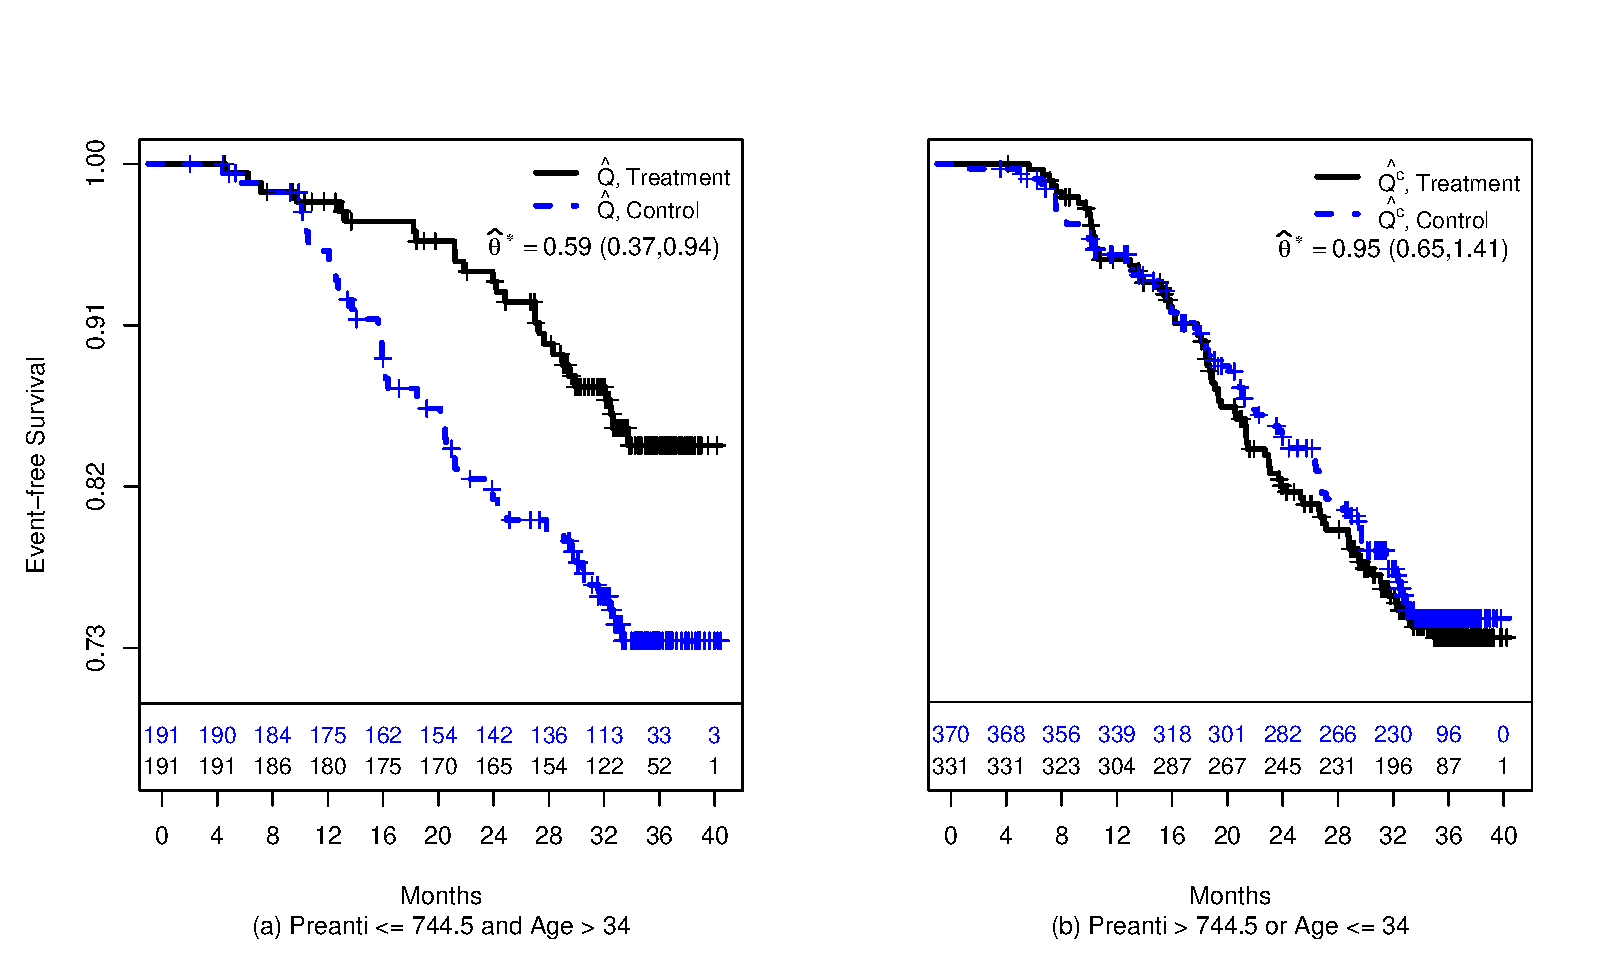
\includegraphics[width=\textwidth, height=3.25in]{Figure 4.eps}
\end{center}
\caption{ACTG-175 analysis application of Forest Search. Kaplan-Meier (K-M) curves (un-adjusted for the estimation of subgroups) with bootstrap-bias corrected 
Cox estimates and $95\%$ confidence intervals denoted $\hat\theta^{*}$: (a) Forest Search $\widehat{Q}$ subgroup; (b) Forest Search $\widehat{Q}^{c}$ subgroup.}
\label{fig:KM_actg}
\end{figure}

\subsection{ACTG-175 analysis}

In our second application we analyze subjects' outcomes from the AIDS Clinical Trials Group Protocol 175 study\cite{ACTG175} which is publicly available in the \R{} \verb+speff2trial+ package \cite{speff2trialR}.  Here our goal is to identify whether a subgroup exists with a pronounced treatment benefit.  We consider the comparison of the combination treatment regimen, zidovudine and didanosine (experimental), to the monotherapy didanosine (control) treatment regimen ($N= 1083$). The Cox ITT hazard ratio estimate  was $0.84$ ($0.65$, $1.09$).  

For the evaluation of a marked treatment benefit we switch the roles of treatment to identify a detrimental effect for control which would correspond to a potentially substantial benefit for the experimental treatment.  We then simply invert the hazard ratio estimates.  For the FS consistency selection criterion we select the largest subgroup with a consistency rate of at least $90\%$.  That is, we are searching for the largest subgroup that is "highly consistent with benefit".  To this end we set the screening threshold in Step 3(a) to $\log(1/0.6)$  and the consistency threshold in Step 3(b) to $\log(1/0.8)$. Cox hazard ratio estimates for candidate subgroups are therefore $\leq 0.60$ and random splits are $\leq 0.8$ in favor of treatment.  We denote the estimated subgroups by $\hat{Q}$ and $\hat{Q}^{c}$ (as opposed to $\hat{H}$ and $\hat{H}^{c}$).

The survival outcomes were defined as the first occurence of three events: A decline in subjects' CD4 T cell count of at least 50; An event indicating progression to AIDS; or death. We consider the following $p=15$ baseline covariates: \verb+Age+, \verb+Wtkg+, \verb+Karnof+ (Karnofsky score), \verb+Cd40+, \verb+Cd80+, \verb+Hemo+ (hemophilia), \verb+HA+ (homosexual activity), 
\verb+Drugs+ (history of IV drug use), \verb+Race+, \verb+Gender+, \verb+Oprior+ (prior non-zidovudine antiretroviral therapy), 
\verb+Symptom+, \verb+Preanti+ (days of prior antiretroviral therapy), \verb+Str2+ (0=naive antiretroviral history,1=experienced), and \verb+Z30+ (zidovudine 30 days prior to study). 

There were 9 categorical (binary) factors, and six continuous factors which were each split (binary cuts) at the mean, 
median, 1st quartile ($q_1$), and 3rd quartile ($q_3$). For GRF candidate selection we 
used $\tau \approx 27$ months for the truncation point and a $2$ month RMST criterion (benefit of $2$ months in favor of control); the $2$ month threshold was chosen as a reasonable criterion since the ITT upper bound for RMST was $\approx 1.5$ months (in favor of control).   The resulting (GRF) candidate factors were \verb+Wtkg<=68.04+, \verb+Age<=29+, and \verb+Preanti<=406+.  For the six continuous factors there were 4 binary cuts (mean, median, $q_1$, and $q_3$) with overlap  for \verb+Age<=29+ (selected by GRF which corresponds to $q_1$), and for \verb+Karnof+ there were 2 cuts (since $q_3$ and the median were redundant). There were thus $K=33$ factors: $9$ categorical, plus $6*4$ ($6$ with 4 binary cuts), plus $3$ per GRF, minus the 3 redundant factors (2 for \verb+Karnof+ and overlap with \verb+Age<=29+).  In total, there were $L = 66$ single factor subgroups with $L(L-1)/2+L = 2,211$ possible subgroups (two-factor combinations); among these subgroups the number of candidates with sample sizes $\geq 60$ and at least $10$ events in each arm was reduced to $1,635$. 

The largest subgroup with a consistency rate of at least $90\%$ was the subgroup formed by the combination of \verb+Preanti<=744.5+ and \verb+Age>34+ (consistency rate
$\approx 92.8\%$).  That is, subjects older than $34$ years (median) and with prior antiretroviral treatment for less than $\approx 2$ years ($q_3$) are estimated to potentially derive ``consistent benefit''.  The resulting $\widehat{Q}$-estimates were $\hat\theta(\widehat{Q}) = 0.52$ ($0.32$,$0.84$) and (bootstrap bias-corrected) $\hat\theta^{*}(\widehat{Q}) =0.59$ ($0.37$, $0.94$).  For the complement, $\hat\theta(\widehat{Q}^{c}) = 1.05$ ($0.77$, $1.44$) and $\hat\theta^{*}(\widehat{Q}^{c}) =0.95$ ($0.65$, $1.41$). The bias-corrected estimate $\hat\theta^{*}(\widehat{Q})$ suggests a relatively strong benefit ($0.59$ vs $0.84$ for ITT) that is statistically significant and corresponds to $382/1083 \approx 35\%$ of the ITT population. Figure \ref{fig:KM_actg} displays the Kaplan-Meier curves for 
the estimated subgroups.


For the $N$-fold cross-validation, across all $N=1083$ training sets there was
a subgroup identified wherein the full analysis subgroup $\widehat{Q}$ 
definition, \verb+Preanti<=744.5+ and \verb+Age>34+, were reproduced for all except 7 (Note that 
$q_3$ for \verb+Preanti+ slightly varied between the training sets and the full analysis, within 1 digit). 
In total $n=386$ subjects ($N$-fold predicted) were classified as $\widehat{Q}$, versus $n=382$ for the full analysis. Interestingly the Cox model estimate for the $N$-fold predicted subgroup 
$\widehat{Q}$ was $0.59$ ($0.37, 0.94$) which is identical to the (bootstrap bias-adjusted) full analysis $\hat\theta^{*}(\widehat{Q}) =0.59$ ($0.37$, $0.94$). For the complement, the $N$-fold predicted subgroup $\widehat{Q}^{c}$ was $1.01$ ($0.73, 1.38$) which is similar to the full analysis $\hat\theta^{*}(\widehat{Q}^{c}) =0.95$ ($0.65$, $1.41$).

Across $200$ random 10-fold cross-validation analyses the median number of training sets (10 folds) where a subgroup is identified 
was 9 out of 10 (The minimum was 7/10 with lower and upper quartiles of $\approx$ 9/10 and 10/10, resp.) resulting in a (median) 
sensitivity of $sensCV(\widehat{Q}) \approx 69\%$.  That is, among the $\widehat{Q}$-classified subjects based on the full analysis the median percentage also $\widehat{Q}$-classified in the (10-fold) cross-validation testing samples was approximately $69\%$.  The median positive predictive value was $ppvCV(\widehat{Q}) \approx 71\%$. For the complement $\widehat{Q}^{c}$, the medians for $sensCV$ and $ppvCV$ were $84\%$ and $83\%$, respectively.  In addition, across the $200$ random 10-fold cross-validation analyses, the full analysis $\hat{Q}$ subgroup factors (cuts) of \verb+Preanti+ and \verb+Age+ appeared in (a median of) $70\%$ and $60\%$ of the training sample 
subgroup definitions, respectively (and jointly in $60\%$).  

The computational timing for the current analysis on an Apple studio (M1 20 core with 69 GB) was approximately: $0.2$ minutes for the FS analysis; $30$ minutes for the $2000$ bootstraps; $22$ minutes for the $N$-fold cross-validation; and $105$ minutes for the $200$ random 10-fold cross-validation analyses.  In total, the number of minutes was $\approx 157$.

In Supplementary materials \textcolor{blue}{S2.2-S2.4} we provide additional analyses.  In particular, we artificially add $20$ standard normal baseline factors as random noise candidates where the FS algorithm does not include lasso in \textcolor{blue}{S2.3}, while in \textcolor{blue}{S2.4} lasso is included.  When lasso is not included (\textcolor{blue}{S2.3}) FS identified a nonsensical subgroup based on a random noise factor. In contrast, when lasso 
is included (\textcolor{blue}{S2.4}) the same subgroup as the full analysis above and (essentially) the same bootstrap bias-adjusted estimates were obtained.  However, $N$-fold CV discrepancies suggest an underlying instability in the presence of including the $20$ random noise factors.

Evaluating the plausibility of the subgroups is hampered by direct access to summaries by the combination of prior antiretroviral therapy duration (\verb+Preanti+) and age in the literature.  However, the role of prior antiretroviral therapy duration viz-a-viz naive-vs-experienced is an important aspect and frequently a key component of regimens studied: Katzenstein et al\cite{Katzenstein_2001} write ``Based on studies of HIV RNA suppression and the development of drug resistance, the goals of antiretroviral treatment in HIV infection have rapidly shifted to early suppression of HIV replication to the lowest possible levels with combination antiretroviral therapy regimens.''
The HIV Trialists' Collaborative Group (HIVTCG) conducted a patient-level meta-analysis (including the ACTG-175 study) of randomized trials:\cite{HTCG_1999} In reference to the combination of zidovudine and didanosine, ``there appeared to be greater effects on the rate ratio for death and disease progression among participants who, at baseline, had either no previous antiretroviral therapy or higher CD4-cell counts.''  Now, for the $\widehat{Q}$ subgroup (\verb+Preanti<=744.5+ and \verb+Age>34+) consisting of $n=382$ subjects there were $46.9\%$ who were antiretroviral treatment naive; for whom the (estimated) enhanced benefit may be plausible in view of the aforementioned HIVTCG analysis. For the remaining $53.1\%$ of subjects, of whom, approximately $91\%$ had zidovudine use in the 30 days prior to treatment initiation and a mean prior antiretroviral therapy duration of $352$ days 
at baseline (mean [median] baseline CD4 count of $324$ [$320$], min = $70$, max = $702$).  Consequently, for these subjects, initiation of the combination of zidovudine and didanosine generally amounted to the {\it continuation} of zidovudine while adding didanosine after (on average) less than a year of prior antiretroviral therapy.  We conjecture the recent zidovudine exposure/experience (as well as ``moderate prior antiretroviral therapy duration")  with the addition of didanosine may have helped with (subsequent) tolerability of the combination and with resistance; however this is just conjecture as we are not aware of available subgroup summaries that are directly applicable.  

\subsection{Supplementary analyses}
As described above, additional analyses of the GBSG and ACTG-175 trials are available in the Supplementary materials \textcolor{blue}{S2.1-S2.4}.  Supplementary materials 
\textcolor{blue}{S2.5} also provides analysis of the systolic heart failure data\cite{Hsich_2011} available in the \verb+randomForestSRC+\cite{Ishwaran_2008} package (a larger trial with $N=
2,231$ subjects, $p = 38$ baseline covariates, and $K=78$); in addition, we induce computational challenges by adding $100$ noise factors and discuss mitigation approaches when the resulting number of subgroup candidate factors is large, $K=379$.
We note that our code implements parallel computing via the \verb+doFuture+\cite{Bengtsson_2021} package for the bootstrapping and CV procedures; accordingly the timing of computations depends on the number of available cores.










\section{Discussion} \label{sec:discuss}

We have proposed a relatively simple and transparent approach for subgroup identification based on Cox hazard ratio estimation criteria indicative of detrimental effects.  We utilize optional GRF and lasso procedures for selecting candidate factors (binary splits) which are the basis for defining subgroups.
GRF is itself a subgroup identification procedure which targets RMST, whereas our use of lasso is for Cox model covariate (prognostic) selection.  In general, any well-defined algorithm can be implemented such as (pre-defined) clinical, and health technology assessment\cite{Agboola_2023} considerations and/or various machine learning algorithms for censored data.  In applications, choices for components of the FS algorithm may be better suited than others.  In particular, in our simulations we found the lasso to help mitigate false-discovery when analyses include baseline factors that are completely random noise. However such random noise seems extreme in clinical trials when baseline factors generally have some degree of prognostic value; nevertheless, the lasso may aid in algorithmic stability.  In addition, whether to maximize the consistency rate or to choose the largest subgroup with a high consistency rate (e.g., at least $90\%$) may differ in stability.  While the proposed CV evaluation cannot establish optimality of a chosen algorithm, it can discern between the quality and stability of algorithms.  The bootstrap bias-correction and variance estimation procedure for the resulting FS Cox hazard ratios would incorporate the chosen algorithm; however if several FS algorithms are evaluated this (exploratory) iterative aspect would not be taken into account.  

The operating characteristics for scenarios/criteria of interest can be quickly approximated via equation (\ref{pHat_approx}). For example if looser/tighter control of the type-1 error is desired the screening and splitting consistency thresholds can be adjusted.  In our simulations we have found the screening and splitting consistency thresholds of $1.25$ and $1.0$ (resp.) have good operating characteristics for identification as well as estimation.  The splitting consistency criteria is similar in spirit to cross-validation, however in contrast to prediction, our relatively simpler goal is to have independent assessments for evidence of harm which is provided by both independent random splits having hazard ratio estimates $\geq 1.0$ across repeated sample splitting.  

Our main application is subgroup analyses for survival outcomes.  In oncology applications the gold-standard primary analysis is the Cox model\cite{FK_2019} usually stratified by randomization stratification factors.  To simplify we have considered the basic Cox model analysis with only the treatment arm as a covariate which is commonly used in oncology forest plot analyses; and is the ``most common approach to analysis''.\cite{ACR_2015}  However, adjusted Cox models\cite{Loh_2018} can also be used either by stratification, direct covariate adjustment (with care to account for any subgroup redundancies in the model) or propensity score-weighting.\cite{Cole_2004}  In addition to bootstrap bias-corrected Cox model estimates, other summaries can also be provided such as RMST and Kaplan-Meier survival curves (e.g., across pre-defined timepoints).  For these summaries the bias-correction and variance estimation procedure described for the Cox model hazard ratios can be applied in an analogous manner.

With our basic Cox model analysis we are targeting marginal hazard ratio effects, which as Aalen et al\cite{ACR_2015} describe can be quite different than the {\it controlled direct effect (CDE)} of treatment.  In their simulation study (See Table 1\citealp{ACR_2015}) the basic Cox model was biased (over-estimated) for the ITT analysis in the presence of a single binary covariate factor which was ``a highly influential risk factor'' (Cox regression effect of $\log(4)$ = $1.386$).   In our simulations the largest discrepancy between the marginal and CDE effects, $\theta^{\dagger}(\cdot)$ vs $\theta^{\ddagger}(\cdot)$, were under model $M_3$ where $\theta^{\dagger}(H)= 2.0$, $\theta^{\ddagger}(H)=2.56$, $\theta^{\dagger}(H^{c})= 0.56$, and $\theta^{\ddagger}(H^{c})=0.49$.   The largest covariate effect under $M_3$ was $\beta_{5}= 0.782$ corresponding to the binary factor $Z_4$ in model (\ref{dgm0}).   Under $M_3$ the \% relative bias and coverage of $\hat\theta^{*}(\widehat{H})$ for $\theta^{\ddagger}(\widehat{H})$ was approximately $-11.6 \%$ and $89\%$. 

While subgroups corresponding to the maximum (detrimental) hazard ratio estimate will generally be subgroup candidates, the proposed consistency criteria for identification does not necessarily correspond to the maximum.  Recent work by Guo et al\cite{GH2021,GW2023} (see also Wang and He\cite{WangHe_2023}) considers de-biased inference for subgroups corresponding to the maximum (best-selected subgroup) treatment estimate.  However, their approach is not an identification procedure per se but utilized for inference via bootstrap calibration when a limited set of subgroups are examined; in their simulations a maximum of 12 pre-specified subgroups are considered, whereas in our three applications (simulated and two real data) the number of subgroups meeting the FS criteria was 70, 263, and $1,635$, respectively.  Zhao et al\cite{Zhao_2023} employ the aforementioned bootstrap calibration\cite{GH2021} in their subgroup identification approach for non-censored continuous outcomes with candidate subgroups estimated via penalized regression with a maximum of $2N$ candidate subgroups through thresholding (in our setup, $K=N$, $L=2N$).    


In our simulation setting the FS and $\grfb$ approaches generally outperform the virtual twins approach in terms of controlling the type-1 error, power, and classification accuracy.  
The virtual twins analyses compared survival differences at 24 and 36 months while $\grfb$ evaluated RMST over a median horizon of $48$ months (range of $33$-$50$) 
and $\grfa$ compared survival differences over a median of $79$ months (range of $55$-$84$).  In contrast the FS approach based on the Cox model conducts comparisons 
across the entirety of follow-up.  We have considered $\grfb$ due to the fairly heavy censoring which, generated by a Weibull model based on the observed \gbsg{} data, depended on covariates with an overall censoring rate of approximately $46\%$.  

The FS approach had favorable performance overall in view of the elevated type-1 errors for GRF, especially under models $M_1$ and $M_2$. When random noise factors were included in the analyses the GRF approach was more susceptible to falsely identifying subgroups.  The $\fsl$ approach was the most stable with a slight decrease in performance, while $\fslg$ inherits an increased type-1 error by the utilization of $\grfb$, but to a much lesser extent than $\grfb$ itself.  Under $M_3$, 
when there was the strongest ITT treatment effect under the null, the type-1 errors for GRF were dramatically decreased (from $\approx 60\%$ to $13\%$ under $M_3$).  Under the nulls of $M_1-M_3$ the ITT treatment differences with respect to RMST were $\approx$ $7.2$, $7.4$, and $11.5$ months.  The ITT Cox marginal effects $\hplimitt$ were $\approx 0.7$ under $M_1$ and $M_2$ and $0.55$ under $M_3$.   While $\hplimitt$ values in the range of $0.55$ is plausible, it seems 
more prudent to consider $\hplimitt$'s in the range of $0.7$ as more realistic in most oncology trials.  Accordingly, although a limited simulation study, the FS approach may strike a more favorable balance between falsely identifying subgroups and reasonable accuracy when large subgroup effects are present.  In terms of estimation, the $\fslg$ bootstrap bias-corrected estimators tend to be conservative: Under-estimating both $\hplim$ and $\Hhplim$ (``conservative for harm'') while over-estimating both $\hcplim$ and $\Hhcplim$ (``conservative for benefit''), except for under model $M_3$ where the relative bias for $\Hhcplim$ was $\hat{b}^{\ddagger} \approx -4.8 \%$.   Though conservative, the coverage rates for $\hchatB$ were $\geq 93\%$ for each target, and the oracle coverage rates $\hat{C}^{oracle}$ for $\hhatB$ and $\hchatB$ were $\geq 95\%$. That is, the bias-corrected versions of $\widehat{H}$ and $\widehat{H}^{c}$ covered ($\geq 95\%$) their respective oracle counterparts.

In principle our approach is exploratory and could be used to guide future trial development.  We believe exploratory subgroup 
identification is valuable even when pre-specified subgroups are of interest (e.g., biomarkers).  As Zhao et al\cite{ZSE2022} write ``A priori subgroup analyses are
free of selection bias and are frequently used in clinical trials and other observational studies. They do discover some effect modification, often convincingly, from the data, but since the potential
effect modifiers are determined a priori rather than using the data, many real effect modifiers may remain undetected''.  In our data analysis applications we consider available data sources to evaluate the plausibility of our subgroup findings.  Patient-level meta-analyses of randomized trials\cite{Davies_2011,HTCG_1999} seems the most feasible and robust avenue for independent `validation' of subgroup results.  However in clinical trials investigating novel therapies/indications there may not be directly relevant data sources available.  The consideration of observational (e.g., real-world data) 
sources could be helpful; see Wang et al\cite{Wang_2023,Sheldrick_2023} for a recent example and methods for utilizing insurance claims databases.  While not an independent (external) evaluation, the proposed cross-validation assessments provide some (internal) diagnostic value.

The subgroup findings from our analyses of the breast cancer and HIV trials could inform patient consultation.  In the breast cancer trial, comparing hormonal therapy (tamoxifen) to chemotherapy, 
the estimated (bias-corrected) hazard ratio for subjects with positive estrogen levels (representing approximately $88\%$ of the study population) was $0.64$ ($0.44$, $0.93$) which suggests a slightly stronger benefit relative to the ITT population ($0.64$ vs $0.69$). Though not dramatic, this could 
increase patients' confidence ("relative to ITT"); in contrast, patients with zero estrogen may want to consider alternatives (We note tamoxifen with low levels of estrogen seems controversial.\cite{Manna_2016,Yu_2021}).  In the HIV trial, comparing the combination of zidovudine and didanosine to monotherapy didanosine, the benefiting subgroup was generally comprised of subjects who were treatment naive or who had recent zidovudine use (within 30 days of study treatment initiation) but with less than a year of prior antiretroviral therapy.  For these subjects, the estimated hazard ratio of $0.59$ ($0.37$, $0.94$) was relatively more substantial compared to the estimated hazard ratio of $0.84$ for the ITT population.
In terms of future trials, these findings could inform study designs such as inclusion criteria (e.g., consider excluding subjects with zero estrogen levels from tamoxifen trials) and/or randomization stratification factors, as well as testing strategies (e.g., pre-specify testing in the [zidovudine plus didanosine] benefiting subgroup described above).  However, in general, we would caution against extrapolating 
findings to comparisons of regimens besides the control regimens that were studied in the trials.

 
Subgroup analyses in Phase 2 trials can be the most actionable and impactful to inform Phase 3 study designs and analyses including: testing strategy; randomization stratification factors; and forest plot subgroup specifications. 
In particular, if there exists a sub-population that could potentially be harmed then identification in Phase 2 could mitigate the risk in later development (e.g., by implementing exclusion criteria/recommendations).  Realistically, only substantial heterogeneous treatment effects can be identified and well estimated in Phase 2 settings; nevertheless, our simulation results under models $M_{2}$ ($N=500$) and $M_{3}$ ($N=300$) suggests potential.
On the other hand, in Phase 3 registrational trials the pre-specified subgroup (forest plot) results may suggest potential lack-of-benefit in a subgroup.\cite{AT_2021}  A comprehensive evaluation of subgroups, targeting large effects, 
may reveal a more accurate characterization than the pre-specified subgroups.  Additionally, in multi-regional clinical trials the establishment of consistency\cite{YSS_2018} can be challenging; the identification of marked subgroup effects 
 in the global trial could inform the evaluation of independent regional trials.
 
Future work will be to extend the inclusion of GRF to additional machine learning methods for censored data so that ``a collection of machine learning'' approaches for FS candidate selection could be evaluated; where regardless of the (algorithmic) source of candidate selection, the resulting FS estimation is in terms of the proposed bootstrap bias-corrected Cox model.   
While our bootstrap bias-correction and variance estimation appears to work well, it would be interesting to evaluate the applicability of the Guo et al\cite{GH2021} bootstrap calibration procedure to our setting which generally involves a large collection of subgroup candidates.

 

\section{Acknowledgements}  The authors wish to thank colleagues Nan Xiao, Jing Zhao, Andy Liaw, and Guoqing Diao for helpful discussions. Comments and suggestions 
from two anonymous referees greatly improved the paper. 

\section{Data Availability Statement}
The data analyzed in the applications is publicly available.  R code for replicating the real data analyses is available at the GitHub repository: 
\href{https://github.com/larry-leon/forestSearch}{https://github.com/larry-leon/forestSearch}.  Additional details and analyses are provided in the Supplementary materials.


\bibliography{subgroups_ref}


\input{tables}


\end{document}


